%%%%%%%%%%%%%%%%%%%%%%%%%%%%%%%%%%%%%%%%%%%%%%%%%%%%%%%%%%%%%%%%%%%%%%%%%%%%%%%%%%%%%%%%%
% Khóa luận tốt nghiệp/Tiểu luận 
% LaTeX Template
% Phiên bản 1.0 (tạo ra ngày 05/10/2022)
% Edited &Modified by VietNC ngày 12/12/2022
%
% Template này có thể được download tại:
% https://github.com/vietnc/HUS-template
% https://github.com/cpc1996/HUS-Dissertation-Template
% 
%
% Phiên bản 1.0 được chỉnh sửa bởi:
% Công Phương Cao (congphuongcao_t59@hus.edu.vn)
% Nguyễn Cảnh Việt (vietncp@gmail.com)
% Nguyễn Tiến Cường (ngtiencuong@gmail.com)
%
% Template được tham khảo từ một phiên bản template của:
% Steve Gunn (http://users.ecs.soton.ac.uk/srg/softwaretools/document/templates/)
% Sunil Patel (http://www.sunilpatel.co.uk/thesis-template/)
%
%%%%%%%%%%%%%%%%%%%%%%%%%%%%%%%%%%%%%%%%%%%%%%%%%%%%%%%%%%%%%%%%%%%%%%%%%%%%%%%%%%%%%%%%%
%----------------------------------------------------------------------------------------
%	(KHÔNG CHỈNH SỬA PHẦN NÀY)
%
%	PHẦN 1: CÁC PACKAGE CƠ BẢN VÀ CÁC TÙY CHỈNH VĂN BẢN
%----------------------------------------------------------------------------------------
%----------------------------------------------------------------------------------------
%	(KHÔNG CHỈNH SỬA PHẦN NÀY)
%
%	PHẦN 1: CÁC PACKAGE CƠ BẢN VÀ CÁC TÙY CHỈNH VĂN BẢN
%----------------------------------------------------------------------------------------

\documentclass[
12pt,
oneside,
english,
doublespacing,
nolistspacing,
liststotoc,
parskip,
headsepline,
chapterinoneline,
]{MastersDoctoralThesis}

% \usepackage[utf8]{inputenc} 
\usepackage[utf8]{vietnam} 
%\usepackage[T1]{fontenc}

\usepackage{mathptmx}
\usepackage{amsmath}
\allowdisplaybreaks

%https://www.overleaf.com/learn/latex/Biblatex_citation_styles
%\usepackage[backend=bibtex,style=authoryear,natbib=true]{biblatex}
\usepackage[backend=bibtex,style=numeric,citestyle=ieee,natbib=true]{biblatex}

\addbibresource{main.bib}

\usepackage[autostyle=true]{csquotes}


%----------------------------------------------------------------------------------------
%	PHẦN 2: CÁC PACKAGE BỔ TRỢ THÊM VÀO TRONG QUÁ TRÌNH BIÊN SOẠN
%----------------------------------------------------------------------------------------

\RequirePackage{setlst}		% Liệt kê/trích dẫn code

\usepackage{multirow}
\usepackage{subfigure}
\usepackage[fontsize=13pt]{scrextend}

%https://www.sascha-frank.com/latex-font-size.html
%https://tex.stackexchange.com/questions/103286/how-to-change-section-subsection-font-size
\usepackage{titlesec}

\titleformat{\section}
{\normalfont\fontsize{13}{13}\bfseries}{\thesection}{1em}{}

\titleformat{\subsection}
{\normalfont\fontsize{13}{13}\bfseries\itshape}{\thesubsection}{1em}{}

%https://tex.stackexchange.com/questions/351961/how-to-indent-code-in-beginverbatim
\usepackage{fancyvrb} 		% Fancy Verbatim
\fvset{tabsize=4,vspace=0pt,fontsize=\footnotesize}

\usepackage{longtable} 		% Bảng dài - Long table

\usepackage[figuresright]{rotating} % Bảng ngang - Sideways table
\usepackage{tabularx}

\usepackage{fontawesome5} 	% Các biểu tượng, ký hiệu đặc biệt

\usepackage{tikz} 			% Vẽ hình
\usepackage{indentfirst}
\setlength{\parindent}{0.5cm}	%Thut dau dong cho doan van
\setlength{\parskip}{1.4ex plus 0.5ex minus 0.3ex}		% Tạo khoảng trống giữa 2 đoạn văn %spacing between two paragraph

\usetikzlibrary{calc}
%----------------------------------------------------------------------------------------
%	PHẦN 3: THÔNG TIN VỀ Khóa luận tốt nghiệp/Tiểu luận (THESIS INFORMATION)
% 	Điền thông tin của các bạn trong file(2.thesis-information) này 
%----------------------------------------------------------------------------------------
%----------------------------------------------------------------------------------------
%	PHẦN 3: THÔNG TIN VỀ Khóa luận tốt nghiệp/Tiểu luận (THESIS INFORMATION)
%----------------------------------------------------------------------------------------
\author{NHÓM 1} 			% Ví dụ: "Nguyễn Thị Thu Thảo"
\thesistitle{ĐIỀU KHIỂN GÓC QUAY ĐỘNG CƠ \\ SỬ DỤNG THUẬT TOÁN PID} % Ví dụ: "Nghiên cứu chế tạo và tính chất quang học của vật liệu nano LaF3:Sm3+"

\supervisor {Đỗ Anh Tuấn} 	% Ví dụ: "PGS. TS. Nguyễn Ngọc Long"
%\supervisorr{Trần Thái Tông} 	% Tên này nếu không có thì để trống!

\field{Học phần: Thực hành hệ thống nhúng} 					% Ví dụ: "Ngành Vật lý", "Ngành Hóa học", v.v.
\program{Lớp K66 - Kỹ thuật Điện tử và Tin học} 			% Ví dụ: "Chương trình đào tạo chuẩn", "Chương trình đào tạo cử nhân tài năng", v.v.
\doctype{Tiểu luận môn học} % Điền vào đây: "Khóa luận tốt nghiệp đại học hệ chính quy" hoặc "Tiểu luận"

\university{\href{http://hus.vnu.edu.vn}{TRƯỜNG ĐẠI HỌC KHOA HỌC TỰ NHIÊN}}
\department{\href{http://hus.vnu.edu.vn/gioi-thieu/co-cau-to-chuc/khoa-truc-thuoc/khoa-vat-ly.html}{KHOA VẬT LÝ}}

\AtBeginDocument{
	\hypersetup{pdftitle=\ttitle}
	\hypersetup{pdfauthor=\authorname}
}

%----------------------------------------------------------------------------------------------------------------------------------------
\begin{document}
\lstset{style=codeC}	% Thiết lập ngôn ngữ C/C++ là ngôn ngữ mặc định cho phần liệt kê souce code của cả bài
\frontmatter 			% Sử dụng hệ thống đánh số La Mã (i, ii, iii, iv...) cho những trang trước phần mục lục
\pagestyle{plain} 
%----------------------------------------------------------------------------------------
%	(KHÔNG CHỈNH SỬA PHẦN NÀY)%
%	PHẦN 4: TRANG TIÊU ĐỀ/TRANG BÌA (TITLE PAGE)
%----------------------------------------------------------------------------------------
% TRANG BÌA CHÍNH:
%----------------------------------------------------------------------------------------
%	(KHÔNG CHỈNH SỬA PHẦN NÀY)
%
%	Phần 6: TRANG TIÊU ĐỀ/TRANG BÌA (TITLE PAGE)
%----------------------------------------------------------------------------------------

% TRANG BÌA CHÍNH:
\begin{titlepage}
	\begin{tikzpicture}[overlay,remember picture]
		\draw [line width=3pt]
		($ (current page.north west) + (2.0cm,-2.0cm) $)
		rectangle
		($ (current page.south east) + (-1.5cm,1.8cm) $);
		\draw [line width=1pt]
		($ (current page.north west) + (2.15cm,-2.15cm) $)
		rectangle
		($ (current page.south east) + (-1.65cm,1.95cm) $); 
	\end{tikzpicture}
	\begin{center}
		
		\vspace{-.04\textheight}
%		\noindent\scshape 			% By CPC
		\noindent 			% Edit by VietNC
		\large \, \href{https://www.vnu.edu.vn/home/}{ĐẠI HỌC QUỐC GIA HÀ NỘI}\\
		\vspace{-0.25cm}{\large \MakeUppercase \univname}\\
		\vspace{-0.25cm}{\large \bfseries \MakeUppercase \deptname}\\[0.5cm]
		
\includegraphics{Logo/Logo_HUS_notext_nocolor}
		
		\vspace{1.0cm}
		
		{\large \MakeUppercase \authorname}
		
		\vspace{2.5cm}
		
		{\Large \bfseries \MakeUppercase\ttitle\par}
		
		\vspace{2.5cm}
		
		{\normalsize \docname\\ \fieldname\\ (\progname)\\}
		
		\vfill
		
		\textbf{Hà Nội - \the\year{}}
	\end{center}
\end{titlepage}


% TRANG BÌA PHỤ:
%----------------------------------------------------------------------------------------
%	(KHÔNG CHỈNH SỬA PHẦN NÀY)
%
%	Phần 6: TRANG TIÊU ĐỀ/TRANG BÌA (TITLE PAGE)
%----------------------------------------------------------------------------------------

% TRANG BÌA PHỤ:
\begin{titlepage}
	\begin{tikzpicture}[overlay,remember picture]
		\draw [line width=3pt]
		($ (current page.north west) + (2.0cm,-2.0cm) $)
		rectangle
		($ (current page.south east) + (-1.5cm,1.8cm) $);
		\draw [line width=1pt]
		($ (current page.north west) + (2.15cm,-2.15cm) $)
		rectangle
		($ (current page.south east) + (-1.65cm,1.95cm) $); 
	\end{tikzpicture}
	\begin{center}
		
		\vspace{-.04\textheight}
%		\noindent\scshape    % By CPC
		\noindent                  % Edit by VietNC
		\large \, \href{https://www.vnu.edu.vn/home/}{ĐẠI HỌC QUỐC GIA HÀ NỘI}\\
		\vspace{-0.25cm}{\large \MakeUppercase \univname}\\
		\vspace{-0.25cm}{\large \bfseries \MakeUppercase \deptname}\\[0.5cm]
		
\includegraphics{Logo/Logo_HUS_notext}
		
		\vspace{1.0cm}
		
		{\large \MakeUppercase \authorname}
		
		\vspace{2.5cm}
		
		{\Large \bfseries \MakeUppercase\ttitle\par}
		
		\vspace{2.5cm}
		
		{\normalsize \docname\\ \fieldname\\ (\progname)\\}
		
		\vspace{2.5cm}
		
		\begin{minipage}[t]{0.49\textwidth}
			\begin{flushright} \large \bfseries
				Giảng viên hướng dẫn:\;
			\end{flushright}
		\end{minipage}
		\begin{minipage}[t]{0.5\textwidth}
			\begin{flushleft} \large \bfseries
				\supname\\
				%\supnamee
			\end{flushleft}
		\end{minipage}
		
		\vfill
		
		\textbf{Hà Nội - \the\year{}}
	\end{center}
\end{titlepage}



\begin{center}
	\bfseries 
	THÀNH VIÊN NHÓM 1
	\mdseries
\end{center}
\begin{enumerate}
	\item Lê Sơn Tùng - 21002243
	\item Lê Trung Kiên - 21002214
	\item Phạm Thu Thủy -  21002240
	\item Từ Văn Hoài Nam - 21002220
	\item Ngô Hoài Nam - 21002219
	\item Trần Tuấn Phong - 21002223
	\item Nguyễn Phan Ngọc Anh - 21002188
\end{enumerate}


%----------------------------------------------------------------------------------------
%	PHẦN 5: DANH NGÔN (QUOTES)
%----------------------------------------------------------------------------------------
%\vspace*{0.2\textheight}

%\noindent\enquote{\itshape 
%	Cái tôi và sự hiểu biết tỷ lệ nghịch với nhau. Hiểu biết càng nhiều cái tôi càng bé. Hiểu biết càng ít, cái tôi càng to.
%}\bigbreak

%\hfill Albert Einstein
%----------------------------------------------------------------------------------------
%	PHẦN 6: LỜI CẢM ƠN (ACKNOWLEDGEMENTS)
%	Các bạn ghi lời cảm ơn vào file(5.ack) này.
%----------------------------------------------------------------------------------------
%----------------------------------------------------------------------------------------
%	PHẦN 6: LỜI CẢM ƠN (ACKNOWLEDGEMENTS)
%----------------------------------------------------------------------------------------

\begin{acknowledgements}
	\addchaptertocentry{\acknowledgementname}
	\thispagestyle{empty}
	
	Lời đầu tiên, nhóm chúng tôi xin được gửi lời cảm ơn chân thành tới thầy Đỗ Anh Tuấn, trong suốt quá trình giảng dạy của môn học, thầy đã truyền tải những kiến thức và giải đáp những thắc mắc của chúng tôi trong môn lập trình nhúng AVR.
	
	Nhóm xin được gửi lời cảm ơn tới các thầy Nguyễn Cảnh Việt và các thầy trong Bộ môn Tin học Vật lý đã luôn tạo điều kiện để chúng tôi được học tập và hoàn thành bài báo cáo này.
	
	Lời cuối cùng, xin được cảm ơn tất cả các thành viên trong nhóm đã không ngại khó khăn, luôn đoàn kết cùng hỗ trợ lẫn nhau để hoàn thành đề tài này
\end{acknowledgements}
%----------------------------------------------------------------------------------------
%	(KHÔNG CHỈNH SỬA PHẦN NÀY)
%
%	PHẦN 7: MỤC LỤC (LIST OF CONTENTS/FIGURES/TABLES PAGES)
%	ĐẶT KHOẢNG CÁCH GIŨA CÁC TIÊU ĐỀ CỦA PHẦN 7
%----------------------------------------------------------------------------------------
\begin{spacing}{1.15}
	\tableofcontents 	% In ra mục lục chính
\end{spacing}

\begin{spacing}{1.15}
	\listoffigures 		% In ra danh sách hình vẽ
\end{spacing}

%\begin{spacing}{1.15}
%	\listoftables		% In ra danh sách bảng
%\end{spacing}

%----------------------------------------------------------------------------------------
%	PHẦN 8: DANH SÁCH TÊN VIẾT TẮT (ABBREVIATIONS)
%
%	Các từ viết tắt các bạn ghi ở đây
%----------------------------------------------------------------------------------------
\begin{abbreviations}{ll} % Thêm danh sách tên viết tắt (dưới dạng một bảng có 2 cột)

\textbf{SP} & \textbf{S}et \textbf{P}oint\\
\textbf{PV} & \textbf{P}rocess \textbf{V}ariable\\
\textbf{MV} & \textbf{M}anipulated \textbf{V}ariable\\
\textbf{e} & \textbf{e}rorr \\
\textbf{P} & \textbf{P}roportional\\
\textbf{I} & \textbf{I}ntegral\\
\textbf{D} & \textbf{D}erivative\\
\end{abbreviations}
%----------------------------------------------------------------------------------------
%%	PHẦN 9: CÁC HẰNG SỐ VẬT LÝ/THÔNG SỐ KĨ THUẬT (PHYSICAL CONSTANTS/OTHER DEFINITIONS)
%%----------------------------------------------------------------------------------------
%\begin{constants}{lr@{${}={}$}l} % Thêm danh sách các hằng số (dưới dạng một bảng có 3 cột)
%
%%	Lệnh \SI{}{} được cung cấp bởi gói siunitx, hãy đọc tài liệu hướng dẫn để biết cách sử dụng nó
%
%%	Tên hằng số 	 & $Biểu tượng$	& $Hằng số$ cùng với đơn vị\\
%	Vận tốc ánh sáng & $c_{0}$		& \SI{2.99792458e8}{\meter\per\second} (chính xác)\\
%
%\end{constants}
%%----------------------------------------------------------------------------------------
%%	PHẦN 10: DANH SÁCH KÝ HIỆU (SYMBOLS)
%%----------------------------------------------------------------------------------------
%
%\begin{symbols}{lll} % Thêm danh sách các ký hiệu (dưới dạng một bảng có 3 cột)
%
%%   Ký hiệu	& Ý nghĩa		& Đơn vị \\
%	$a$		& khoảng cách	& \si{\meter} \\
%	$P$		& công suất		& \si{\watt} (\si{\joule\per\second}) \\
%
%	\addlinespace % Khoảng cách để phân biệt giữa ký hiệu Latin với ký hiệu La Mã
%
%	$\omega$ & tần số góc	& \si{\radian} \\
%
%\end{symbols}

%----------------------------------------------------------------------------------------
%	(KHÔNG CHỈNH SỬA PHẦN NÀY)
%
%	PHẦN 11: LỜI ĐỀ TẶNG (DEDICATION)
%----------------------------------------------------------------------------------------

%\dedicatory{Dành tặng/Dành cho/Gửi tới\ldots} 


%----------------------------------------------------------------------------------------
%	PHẦN 12: NỘI DUNG/CÁC CHƯƠNG Khóa luận tốt nghiệp/Tiểu luận (THESIS CONTENT - CHAPTERS)
%----------------------------------------------------------------------------------------

\mainmatter % Bắt đầu đánh số trang (1,2,3...)

\pagestyle{plain}

% Hãy thêm những chương (chapter) của khóa luận/tiểu luận vào thư mục Chapters
% Hãy bỏ chú thích những dòng nếu bạn đã bổ sung những chương vào

% MỞ ĐẦU (LỜI MỞ ĐẦU - Chương 0)

\chapter*{MỞ ĐẦU} % Tên của chương
\addcontentsline{toc}{chapter}{MỞ ĐẦU} % Thêm tên chương vào mục lục

\label{Chapter0} % Để trích dẫn chương này ở chỗ nào đó trong bài, hãy sử dụng lệnh \ref{Chapter0} 

%----------------------------------------------------------------------------------------

Điều khiển tự động là một lĩnh vực khoa học hiện đại. Hiện nay, ta có thể thấy điều khiển tự động xuất hiện trong nhiều lĩnh vực như: đời sống, công nghiệp, nông nghiệp, năng lượng, giao thông, quân sự... Rõ ràng, điều khiển tự động đóng vai trò quan trọng trong sự phát triển của đời sống cũng như trong cuộc sống thường ngày.

Thuật toán điều khiển hệ thống bắt đầu xuất hiện từ giữa thế kỷ XIX và phát triển mạnh mẽ vào những năm 60 của thế kỷ XX với lý thuyết điều khiển nâng cao. Sự ra đời của chúng giúp con người đạt được nhiều thành tựu to lớn trong nhiều lĩnh vực. Một trong những thuật toán điều khiển vẫn được sử dụng cho đến ngày này đó chính là bộ điều khiển PID. Đây là hệ thống điều khiển phản hồi kiểu vòng kín phổ biến nhất hiện nay với cấu trúc đơn giản, dễ thực hiện và tính hiểu quả cao.

Để làm rõ hơn về bộ điều khiển PID, tiểu luận này sẽ tìm hiểu về thuật toán PID và ứng dụng của nó trong các mô hình thực tế. Nội dung của tiểu luận sẽ được chia làm ba chương như sau: 

\bfseries 
Chương 1: Tổng quan về PID.

Chương 2: Thiết kế hệ thống và thực nghiệm.

Chương 3: Kết luận.
\mdseries
% Chương 1

\chapter{ TỔNG QUAN VỀ PID} % Tên của chương

\label{Chapter1} % Để trích dẫn chương này ở chỗ nào đó trong bài, hãy sử dụng lệnh \ref{Chapter1} 

%----------------------------------------------------------------------------------------

% Định nghĩa một số lệnh cần thiết để điều chỉnh định dạng cho một số nội dung nhất định trong bài
\newcommand{\keyword}[1]{\textbf{#1}}
\newcommand{\tabhead}[1]{\textbf{#1}}
\newcommand{\code}[1]{\texttt{#1}}
\newcommand{\file}[1]{\texttt{\bfseries#1}}
\newcommand{\option}[1]{\texttt{\itshape#1}}

%----------------------------------------------------------------------------------------

\section{Giới thiệu chung}

PID (Proportional Integral Derivative) là một cơ chế phản hồi vòng điều khiển được sử dụng rộng rãi trong các hệ thống điều khiển tự động. Bộ điều khiển PID sẽ tính toán sai số là hiệu giữa giá trị trả về của hệ thống và giá trị điểm đặt mong muốn, từ đó thực hiện giảm sai số về mức nhỏ nhất bằng cách điều chỉnh giá trị điều khiển đầu vào. Để hệ thống đạt được kết quả tốt nhất, các thông số PID sẽ được điều chỉnh theo tính chất, đặc trưng của hệ thống.
 
\section{Cơ bản về vòng điều khiển}

Xét ví dụ về một cánh tay robot có thể điều khiển chuyển động và xác định vị trí của nó. Động cơ điện được sử dụng sao cho khi cấp điện cho động cơ, cánh tay sẽ di chuyển nâng lên hoặc hạ xuống. Khi vận hành, cần điều khiển cánh tay đến một vị trí cụ thể, tuy nhiên việc cấp năng lượng đơn thuần không thể điều khiển cánh tay robot một cách chính xác bởi quán tính, trọng lực, ngoại lực tác động lên nó trong quá trình vận hành (dịch chuyển, nâng vật, hạ vật...). Chính vì thế, ta cần sử dụng một vòng điều khiển để có thể vận hành cánh tay robot với sai số nhỏ nhất có thể.

\begin{itemize}
	
	\item PV (Process Variable): Biến quá trình - vị trí của cánh tay robot.
	\item SP (Setpoint): Vị trí điều khiển mong muốn. 
	\item e (error): Sai số hệ thống, là hiệu giữa SP và PV.
	\item MV (Manipulated Variable): Biến điều khiển, là đầu ra của bộ điều khiển PID.
	
\end{itemize}

Từ việc xác định vị trí hiện tại của động cơ (PV) so với vị trí điểm đặt mong muốn, hệ thống sẽ tính toán sai số, kết hợp với các thuật toán, bộ điều khiển sẽ cung cấp cho động cơ một dòng điện phù hợp để cánh tay robot đạt được vị trí mong muốn.

\section{Cấu trúc của bộ điều khiển PID}
Tiểu luận này trình bày dạng song song của bộ điều khiển PID. Bộ điều khiển PID gồm ba thành phần: tỉ lệ, tích phân, vi phân.

\begin{figure}[h!]
	\centering
	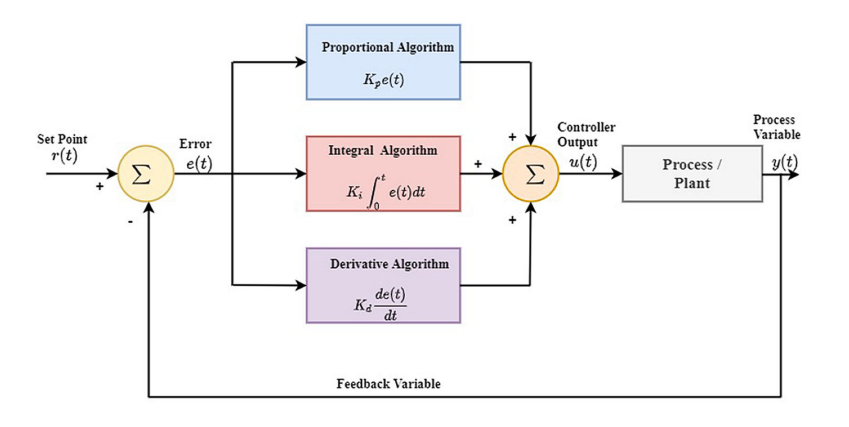
\includegraphics[width=0.8\textwidth]{cau truc pid.png}
	\caption[Cấu trúc của bộ điều khiển PID]{Cấu trúc của bộ điều khiển PID}
	\label{fig:cautrucPID}
\end{figure}

Tổng của ba thành phần này chính là đầu ra của hệ thống(MV).
\begin{align}
 	MV(t) = u(t) &= P_{out} + I_{out} + D_{out}   \\
		&= K_p.e(t) + K_i.\int_{0}^{t}e(t)dt + K_d.\frac{d}{dt}e(t)
\end{align}
    
\subsection{Thành phần tỉ lệ}

Tỷ lệ (Proportional): Làm thay đổi giá trị đầu ra tỷ lệ với giá trị sai số hiện tại. Tuy nhiên trong thực tế, do sự sai lệch nên sẽ không bao giờ đặt được đến giá trị mong muốn. Để đáp ứng tỉ lệ cần nhân sai số với độ lợi $K_p$. Độ lợi tỷ lệ cao dẫn đến sự thay đổi lớn cho đầu ra. Nếu độ lợi tỷ lệ quá cao, hệ thống có thể trở nên không ổn định. Ngược lại, độ lợi nhỏ dẫn đến phản hồi đầu ra nhỏ và bộ điều khiển kém nhạy hơn. Tỷ lệ đóng góp phần lớn sự thay đổi đầu ra.

Thành phần tỉ lệ được cho bởi:
\begin{align}
	P_{out} &= K_p.e(t)
\end{align} 
Trong đó:

\begin{itemize}
	
	\item $P_{out}$: Đầu ra của khâu tỉ lệ.
	\item $K_p$: Độ lợi tỉ lệ(là một tham số điều chỉnh).
	\item e: sai số = SP - PV.
	\item t: thời gian tức thời(hiện tại).
	
\end{itemize}

\subsection{Thành phần tích phân}

Tích phân (Integral): Khâu này tỉ lệ với biên độ sai số và thời gian xảy ra sai số. Cộng dồn các sai số tức thời theo thời gian (tích phân sai số) cho ra tích lũy sai số. Tích lũy sai số sau đó được nhân với độ lợi tích phân $K_p$. Thuật ngữ tích phân tăng tốc độ di chuyển của hệ thống về phía điểm đặt và loại bỏ lỗi trạng thái ổn định còn lại xảy ra với bộ điều khiển chỉ sử dụng thành phần tỉ lệ. Tuy nhiên, việc cộng dồn các sai số tích lũy từ quá khứ của khâu tích phân có thể khiến giá trị hiện tại vượt quá giá trị điểm đặt.

Thành phần tích phân được cho bởi:

\begin{align}
	I_{out} &= K_i.\int_{0}^{t}e(t)dt
\end{align}

Trong đó:

\begin{itemize}
	
	\item $P_{out}$: Đầu ra của khâu tích phân.
	\item $K_i$: Độ lợi tích phân(là một tham số điều chỉnh).
	\item e: sai số = SP - PV.
	\item t: thời gian tức thời(hiện tại).
	
\end{itemize}

\subsection{Thành phần đạo hàm}

Đạo hàm (Derivative): Một thành phần khác được sử dụng trong bộ điều khiển PID là đạo hàm. Tốc độ thay đổi của sai số quá trình được tính toán bằng cách xác định độ dốc của sai số theo thời gian (tức là đạo hàm bậc một theo thời gian) và nhân với độ lợi $K_p$. Đạo hàm dự đoán hành vi của hệ thống từ đó cải thiện ổn định của hệ thống.

Thành phần đạo hàm được cho bởi:

\begin{align}
	D_{out} &= K_d.\frac{d}{dt}e(t)
\end{align}

Trong đó:

\begin{itemize}
	
	\item $D_{out}$: Đầu ra của khâu tích phân.
	\item $K_d$: Độ lợi(là một tham số điều chỉnh).
	\item e: sai số = SP - PV.
	\item t: thời gian tức thời(hiện tại).
	
\end{itemize}







%----------------------------------------------------------------------------------------

\section{Một số bộ điều khiển được xây dựng từ P, I và D}

Tùy vào đặc trưng của một số hệ thống và mục đích sử dụng, có thể kết hợp các thành phần: tỷ lệ (P), tích phân (I) và đạo hàm (D) để tạo nên một số bộ điều khiển.


\subsection{Bộ điều khiển tỷ lệ tích phân}

Bộ điều khiển tỷ lệ tích phân (PI) được xây dựng bằng việc kết hợp hai thành phần tỷ lệ (P), tích phân (I) và không sử dụng thành phần đạo hàm (D) của thuật toán PID. Hệ thống PI là một hình thức kiểm soát phản hồi. Nó cung cấp thời gian phản hồi nhanh hơn so với điều khiển chỉ sử dụng thành phần tích phân (I) do bổ sung thành phần tỷ lệ (P). Điều khiển PI ngăn hệ thống dao động và điều khiển hệ thống về điểm đặt (SP).

\newpage

Đầu ra của bộ điều khiển PI:

\begin{align}
	MV(t) &= P_{out} + I_{out}    \\
	&= K_p.e(t) + K_i.\int_{0}^{t}e(t)dt 
\end{align}

\subsection{Bộ điều khiển tỷ lệ đạo hàm}

Một sự kết hợp khác của hệ thống PID là bộ điều khiển tỷ lệ đạo hàm (PD). Thành phần của bộ điều khiển gồm hai thành phần tỷ lệ (P) và đạo hàm (D), bỏ qua thành phần tích phân (I). Một hệ thống PD hoạt động trên quy trình hiện tại và dự đoán. Đầu ra điều khiển là sự kết hợp tuyến tính của tín hiệu lỗi và đạo hàm của nó.

Đầu ra của bộ điều khiển PD:

\begin{align}
	MV(t) &= P_{out} + D_{out}   \\
	&= K_p.e(t) + K_d.\frac{d}{dt}e(t)
\end{align}


\subsection{Bộ điều khiển tỷ lệ - tích phân - đạo hàm}

Như đã đề cập ở trên, bộ điều khiển PID là sự kết hợp của cả ba khâu: tỷ lệ, tích phân và đạo hàm. Hệ thống PID được sử dụng rộng rãi nhất bởi nó là sự kết hợp các ưu điểm của ba thành phần này. Mỗi thành phần có vai trò đặc trưng giúp cho hệ thống được tối ưu trong quá trình hoạt động và mang lại hiệu suất cao.

\section{Các thành phần độ lợi của hệ thống}
Với cấu trúc đơn giản và hiệu quả mang lại cao mà ngày nay điều khiển PID vẫn được sử dụng rộng rãi trong công nghiệp. Ba hằng số độ lợi: tỷ lệ ($K_p$), tích phân ($K_i$) và đạo hàm ($K_d$) có ý nghĩa quan trọng trong một hệ thống PID. Việc thay đổi các hằng số này sẽ quyết định đến đầu ra của hệ thống. Chính vì thế, một bộ điều khiển PID được "tinh chỉnh tốt" có thể mang lại hiệu suất tuyệt vời. Từ "tinh chỉnh tốt" nhấn mạnh rằng hiệu suất của bộ điều khiển PID chủ yếu phụ thuộc vào quá trình điều chỉnh \cite{aastrom2001future}. Mỗi hệ thống cần có bộ số $K_p$, $K_i$, $Kd$ khác nhau sao cho phù hợp để hệ thống hoạt động ổn định, đảm bảo hiệu suất với bài toán đặt ra.

\subsection{Độ lợi tỷ lệ}

Giá trị của độ lợi tỷ lệ ($K_p$) càng lớn thì hệ thống đáp ứng càng nhanh, tuy nhiên sai số sẽ càng lớn. Một giá trị $K_p$ quá lớn sẽ làm cho hệ thống hoạt động bị sai lệch, thiếu sự ổn định và tin cậy. Ngược lại, nếu $K_p$ quá nhỏ cũng khiến cho hệ thống hoạt động kém nhạy, dẫn đến mất tính ổn định cho toàn hệ thống.

\begin{figure}[h!]
	\centering
	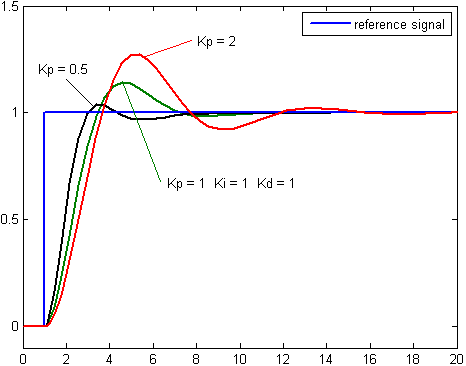
\includegraphics[width=0.8\textwidth]{Kp.png}
	\caption[Đáp ứng khâu tỷ lệ của hệ thống với $Ki$, $K_d$ không đổi]{Đáp ứng khâu tỷ lệ của hệ thống với $Ki$, $K_d$ không đổi}
	\label{fig:Đáp ứng $K_p$}
\end{figure}

\newpage

\subsection{Độ lợi tích phân}

Giá trị của độ lợi tích phân ($K_i$) càng lớn thì sai số ổn định bị triệt tiêu càng nhanh, đổi lại độ vọt lố của hệ thống càng lớn. Các giá trị sai số được tích phân trong quá trình đáp ứng của hệ thống cần phải được triệt tiêu bằng tích phân trước khi tiến tới trạng thái ổn định. 

\begin{figure}[h!]
	\centering
	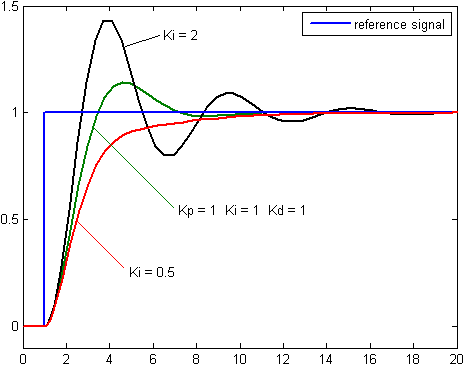
\includegraphics[width=0.8\textwidth]{Ki.png}
	\caption[Đáp ứng khâu tích phân của hệ thống với $Ki$, $K_d$ không đổi]{Đáp ứng khâu tích phân của hệ thống với $Ki$, $K_d$ không đổi}
	\label{fig:Đáp ứng $K_i$}
\end{figure}

\newpage

\subsection{Độ lợi đạo hàm}

Giá trị của độ lợi đạo hàm ($K_d$) càng lớn, độ vọt lố càng giảm nhưng lại làm chậm đáp ứng của hệ thống và có thể dẫn đến sự mất ổn định trong quá trình hoạt động của hệ thống.

\begin{figure}[h!]
	\centering
	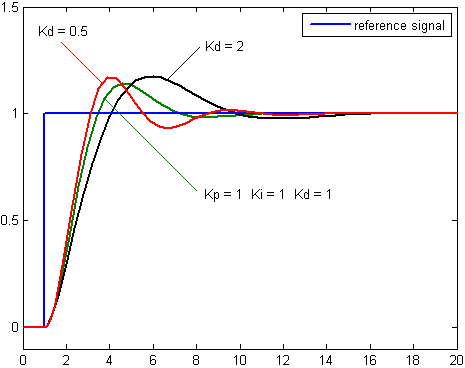
\includegraphics[width=0.8\textwidth]{Kd.png}
	\caption[Đáp ứng khâu đạo hàm của hệ thống với $Ki$, $K_d$ không đổi]{Đáp ứng khâu đạo hàm của hệ thống với $Ki$, $K_d$ không đổi}
	\label{fig:Đáp ứng $K_d$}
\end{figure}

\section{Một số phương pháp điểu chỉnh thông số PID}

Một bộ điều khiển PID phụ thuộc rất nhiều vào ba thông số độ lợi. Nếu ba thông số $K_p$, $K_i$, $K_d$ không được lựa chọn thích hợp, hệ thống sẽ hoạt động với độ tin cậy thấp, độ chính xác kém và dẫn đến sai lệch của hệ thống. Chính vì thế, cần xác định bộ số này sao cho phù hợp với hệ thống. Có nhiều phương pháp để điều chỉnh thông số PID cho một hệ thống.

\subsection{Phương pháp điều chỉnh thủ công}

Đây là phương pháp hiệu chỉnh đơn giản, dễ dàng đạt được một hệ thống có đáp ứng đầu ra như ý muốn và không cần thiết phải có mô hình chi tiết về toán học của hệ thống. Tuy nhiên phương pháp này là mất nhiều thời gian và người hiệu chỉnh cần phải có nhiều kinh nghiệm. Các bước hiệu chỉnh:

\begin{itemize}	
	\item Đầu tiên chỉnh cả ba thông số $K_p$, $K_i$, $K_d$ về 0. 
	\item Tăng dần $K_p$ cho đến khi đầu ra của vòng điều khiển dao động, sau đó $K_p$ được đặt về xấp xỉ một nửa giá trị đó.
	\item Tiếp theo, tăng giá trị $K_i$ đến giá trị phù hợp sao cho hệ thống đủ thời gian xử lý. Tuy nhiên, giá trị $K_i$ quá lớn sẽ gây mất ổn định.
	\item Cuối cùng tăng $K_d$ đến khi dao động của hệ thống bị loại bỏ. $K_d$ quá lớn sẽ khiến đáp ứng dư và vọt lố.
\end{itemize}

\subsection{Phương pháp Ziegler–Nichols 2}
Phương pháp Ziegler–Nichols được đưa ra bởi John G. Ziegler và Nathaniel B. Nichols vào những năm 1940. Các bước hiệu chỉnh bằng phương pháp này bao gồm:

\begin{itemize}
	\item Chỉnh $K_p$, $K_i$, $K_d$ về 0. 
	\item Tăng dần độ lợi $K_p$ từ 0 cho đến khi đạt được độ lợi $K_{cr}$ mà tại đó đầu ra của của vòng điều khiển dao động với biên độ không đổi.
	\begin{figure}[h!]
		\centering
		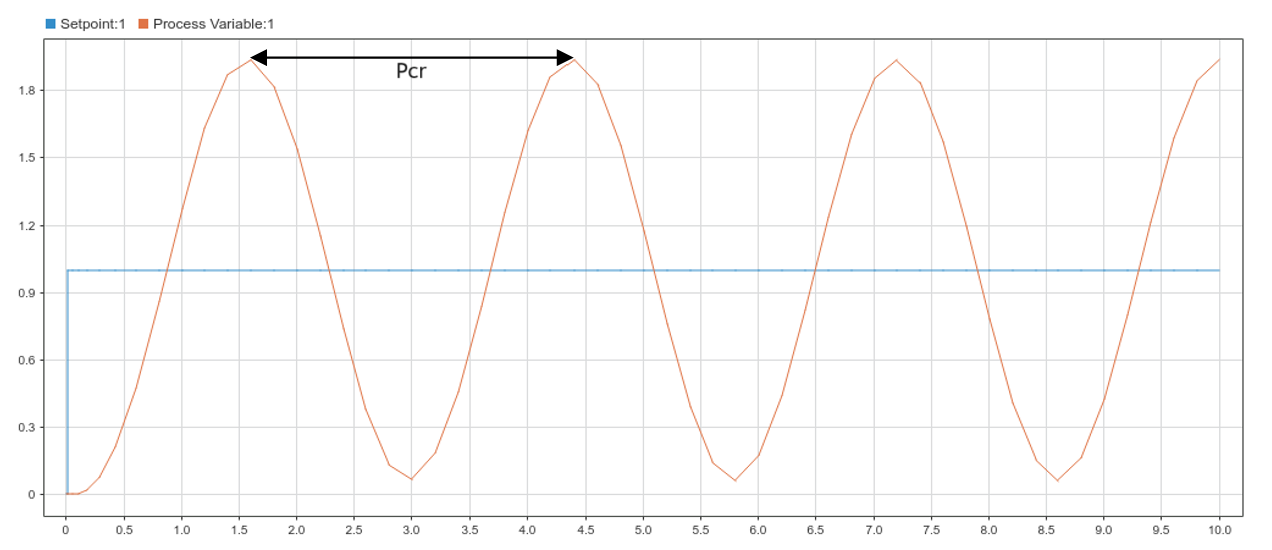
\includegraphics[width=0.8\textwidth]{Pcr.png}
		\caption[Mô tả đầu ra của hệ thống dao động với chu kỳ không đổi]{Mô tả đầu ra của hệ thống dao động với chu kỳ không đổi}
		\label{fig:Dao động của đầu ra hệ thống}
	\end{figure}
	\item Sau khi hệ dao động tuần hoàn, tiến hành xác định chu kỳ dao động $P_{cr}$ của hệ thống. Lưu ý rằng, đơn vị thời gian được lấy theo đơn vị của thời gian lấy mẫu trong hệ thống.
	
	\newpage
	
	\item Từ các giá trị $K_{cr}$ và $P_{cr}$ tìm được, có thể xác định được các giá trị $T_i$ và $T_d$ theo bảng:


	\begin{figure}[h!]
	 	\centering
		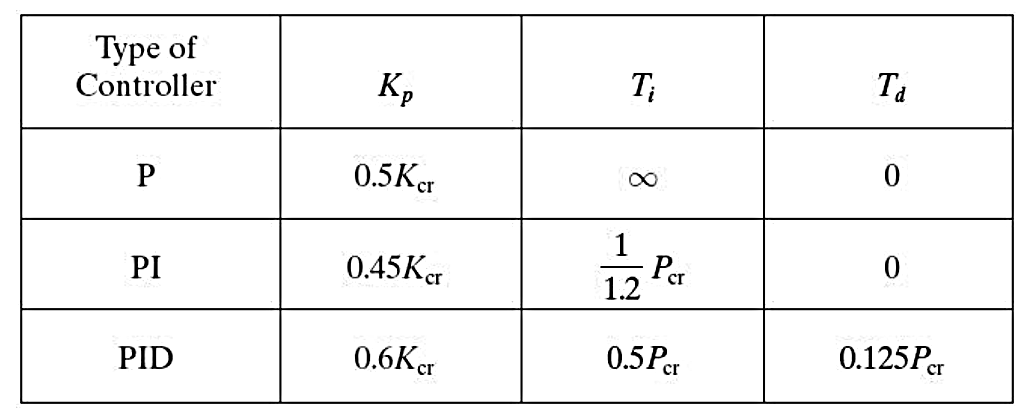
\includegraphics[width=0.8\textwidth]{Ziegler-Nichols.png}
		\caption[Bảng Ziegler-Nichols 2]{Bảng Ziegler-Nichols 2}
		\label{fig:Ziegler-Nichols 2}
	\end{figure}
	
	\item Dựa vào Ziegler-Nichols 2, các thông số $K_i$ và $K_d$ được xác định bởi:
	\begin{align}
		K_i = K_p/T_i	\\
		K_d = K_p.T_d
	\end{align}
	
	
\end{itemize}

\newpage

\subsection{Phương pháp sử dụng phần mềm chuyên dụng}

Đây là phương pháp điều chỉnh chắc chắn, chính xác. Đây là phương pháp giúp tối ưu hóa hiệu suất hệ thống, dễ dàng điều chỉnh và khả năng đáp ứng linh hoạt. Hạn chế của phương pháp này là tốn kém chi phí và cần hiểu rõ về chuyên môn cũng như hệ thống.

Dưới đây là mô tả phương pháp hiệu chỉnh độ lợi bằng cách sử dụng phần mềm Matlab Simulink. Đây là phương pháp mang lại độ tối ưu và tin cậy cao cho hệ thống. Tuy nhiên, để sử dụng phương pháp này thì cần phải đưa ra các phương trình toán học cho hệ thống, đây là một công việc đòi hỏi tính học thuật cao và khá khó khăn.

\begin{figure}[h!]
	\centering
	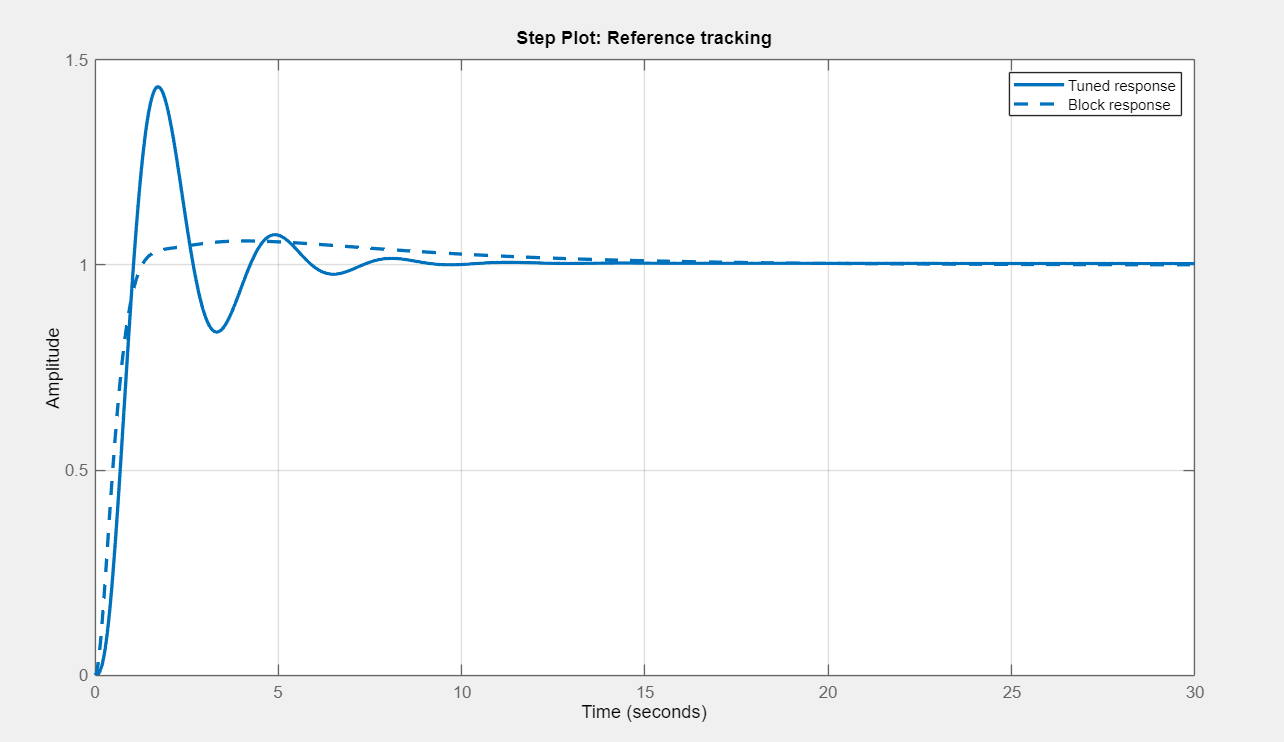
\includegraphics[width=0.8\textwidth]{tuning.png}
	\caption[Bảng hiệu chỉnh độ lợi bằng phần mềm Matlab]{Bảng hiệu chỉnh độ lợi bằng phần mềm Matlab}
	\label{fig:Hiệu chỉnh độ lợi bằng phần mềm}
\end{figure}




% Chương 2

\chapter{THIẾT KẾ HỆ THỐNG} % Tên của chương

\label{Chapter2} % Để trích dẫn chương này ở chỗ nào đó trong bài, hãy sử dụng lệnh \ref{Chapter2} 

%----------------------------------------------------------------------------------------

% Định nghĩa một số lệnh cần thiết để điều chỉnh định dạng cho một số nội dung nhất định trong bài

%\newcommand{\keyword}[1]{\textbf{#1}}
%\newcommand{\tabhead}[1]{\textbf{#1}}
%\newcommand{\code}[1]{\texttt{#1}}
%\newcommand{\file}[1]{\texttt{\bfseries#1}}
%\newcommand{\option}[1]{\texttt{\itshape#1}}

%----------------------------------------------------------------------------------------

\section{Giới thiệu}
Dựa vào lý thuyết của thuật toán điều khiển PID, tiểu luận này đã xây dựng mô hình thực tế có sử dụng bộ điều khiển này đó là mô hình điều khiển vị trí góc quay động cơ DC Encoder.


\section{Điều khiển vị trí góc quay động cơ DC Encoder sử dụng thuật toán PID}

\subsection{Tổng quan}
Bằng việc sử dụng thuật toán điều khiển PID, có thể điều khiển vị trí của động cơ DC Encoder dựa vào đĩa Encoder được gắn sẵn trên trục động cơ. 

\subsection{Lý thuyết}

Sử dụng động cơ DC giảm tốc GA25 Encoder. Động cơ có gắn thêm phần Encoder là một đĩa Encoder 11 xung, hai kênh A và B để có thể trả xung về vi điều khiển. Dựa vào giá trị xung trả về, có thể biết được vị trí hiện tại của đĩa. Từ đó có thể dễ dàng xác định vị trí hoặc vận tốc của động cơ. Cùng với việc sử dụng thuật toán điều khiển PID, vị trí hay tốc độ của động cơ được điều khiển một cách chính xác. 

\begin{figure}[h!]
	\centering
	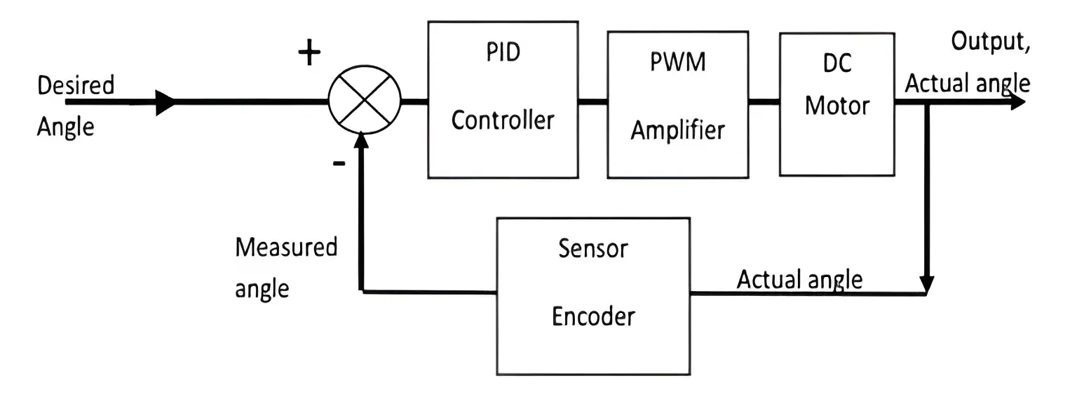
\includegraphics[width=0.8\textwidth]{pid_sd.png}
	\caption[Sơ đồ khối hệ thống]{Sơ đồ khối hệ thống}
	\label{fig:Sơ đồ khối hệ thống}
\end{figure}


\subsection{Một số chức năng được sử dụng trong mô hình}
\subsubsection{Ngắt ngoài - External Interrupt}

Ngắt (interrupt) là những lời gọi hàm tự động khi hệ thống sinh ra một sự kiện. Những sự kiện này được nhà sản xuất vi điều khiển thiết lập bằng phần cứng và được cấu hình trong phần mềm bằng những tên gọi cố định. Ngắt giúp chương trình gọn nhẹ và xử lý nhanh hơn. Ví dụ với việc kiểm tra một nút nhấn có được nhấn hay không, việc kiểm tra trạng thái nút nhấn trong vòng lặp while(1) của chương trình có thể gây ảnh hưởng tới chương trình chính. Với việc sử dụng ngắt, chỉ cần nối nút nhấn đến đúng chân có hỗ trợ ngắt, sau đó cài đặt ngắt sẽ sinh ra khi trạng thái nút chuyển từ HIGH->LOW. Thêm một tên hàm sẽ gọi khi ngắt sinh ra. Như vậy đoạn chương trình ngắt sẽ cho biết trạng thái nút nhấn.

Có bốn trạng thái của ngắt bao gồm:

\begin{itemize}
	
	\item LOW: kích hoạt liên tục khi trạng thái chân digital có mức thấp
	\item HIGH: kích hoạt liên tục khi trạng thái chân digital có mức cao.
	\item RISING: kích hoạt khi trạng thái của chân digital chuyển từ mức điện áp thấp sang mức điện áp cao.
	\item FALLING: kích hoạt khi trạng thái của chân digital chuyển từ mức điện áp cao sang mức điện áp thấp.
	
\end{itemize}

Trong mô hình này việc xác định chiều quay của động cơ sẽ được thực hiện bằng cách sử dụng ngắt INT0 (chân PD2) ở chế độ RISING, kênh A của Encoder được nối với chân PD2, kênh B được nối vào chân PD3. Như vậy mỗi khi ngắt được tạo ra, bằng cách đọc giá trị ở kênh B, có thể xác định được chiều quay của động cơ.

\begin{figure}[h!]
	\centering
	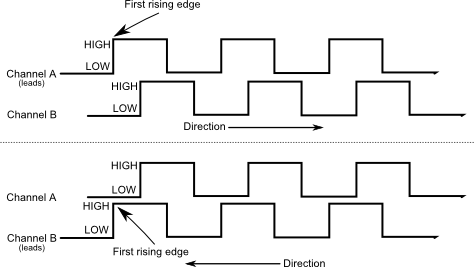
\includegraphics[width=0.8\textwidth]{encoder.png}
	\caption[Xác định chiều quay của động cơ DC Encoder]{Xác định chiều quay của động cơ DC Encoder}
	\label{fig:Xác định chiều quay của động cơ DC Encoder}
\end{figure}
\newpage
\subsubsection{Tạo xung Fast PWM}

\begin{figure}[h!]
	\centering
	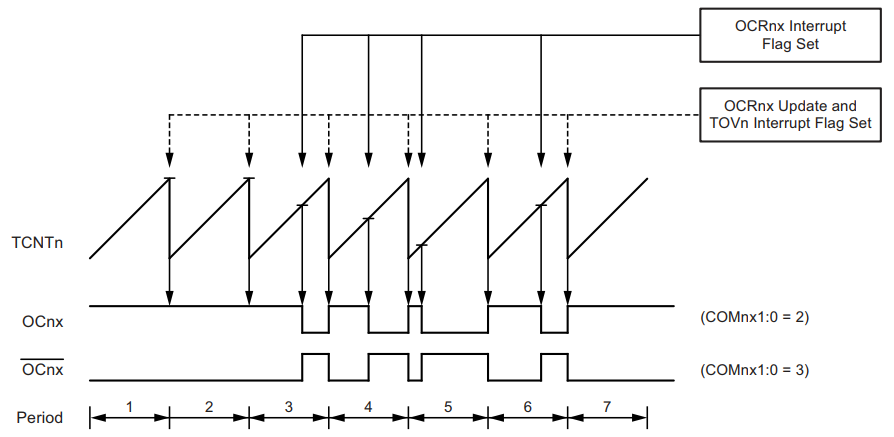
\includegraphics[width=0.8\textwidth]{pwm.png}
	\caption[Tạo xung Fast PWM]{Tạo xung Fast PWM}
	\label{fig:Tạo xung Fast PWM}
\end{figure}

WGM2:0 = 0b011 hoặc 0b111.

Counter chạy từ 0x00 tới TOP rồi được reset lại về 0x00. 

TOP = MAX khi WGM2:0 = 0b011; TOP = OCRxA nếu WGM2:0 = 0b111 

Khi CTNTx = OCRxn, tạo ra phản ứng tại chân OCxn. Phản ứng tại chân OCxn tùy thuộc vào giá trị của bit COMxn1:0
\newpage
Ngắt được tạo ra (nếu cho phép) khi CTNTx  = TOP.

\begin{figure}[h!]
	\centering
	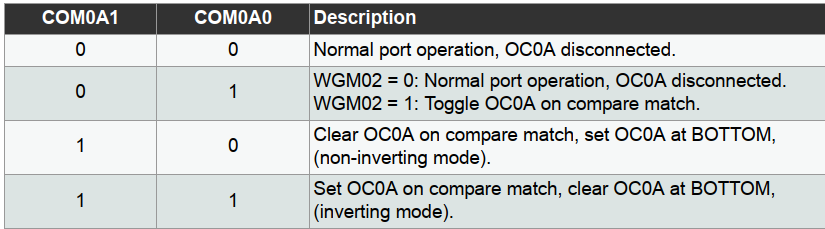
\includegraphics[width=0.8\textwidth]{pwm2.png}
	\caption[Chế độ trong tạo xung Fast PWM]{Chế độ tạo xung Fast PWM}
	\label{fig:Chế độ tạo xung Fast PWM}
\end{figure}

Tần số PWM tại đầu ra OCxn chỉ phụ thuộc vào tần số clock đưa vào Timer.

Giá trị trên thanh ghi so sánh OCRxn quyết định mức năng lượng được kích hoạt trong mỗi chu kì. 

Công thức tính chu kì xung PWM: 

\begin{align}
	f_{OCxA} = \frac{f_{IO}}{2.d.MAX}
\end{align}

Trong đó:
\begin{itemize}
	
	\item d : hệ số chia clock của timer
	\item $f_{IO}$ : Tần số clock của IO
	\item $f_{OCxA}$ : Tần số xung tại đầu ra so sánh OCxA
	
\end{itemize}
\newpage
Như vậy, bằng việc tạo xung Fast PWM, có thể dễ dàng điều khiển tốc độ quay của động cơ thông qua module L298N.

\begin{figure}[h!]
	\centering
	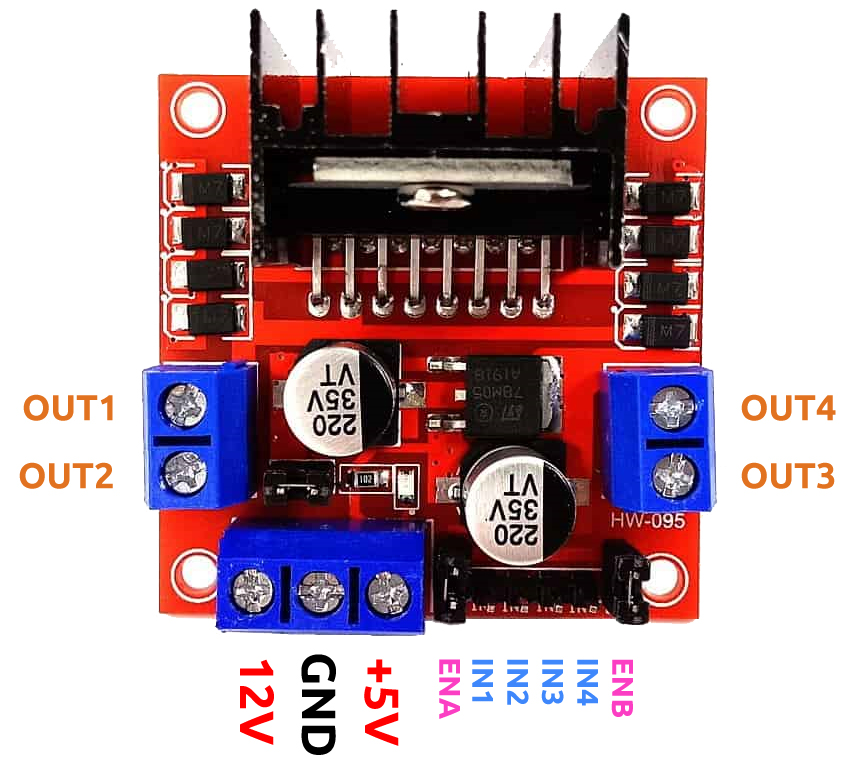
\includegraphics[width=0.6\textwidth]{l298n.jpg}
	\caption[Module L298N]{Module L298N}
	\label{fig:Module L298N}
\end{figure}

Chiều quay của động cơ được thay đổi bằng việc thay đổi giá trị trên chân PD6 nối với IN3 của module và PD7 nối với INT4 của module.
\newpage

\subsubsection{Analog to Digital Converter (ADC)}

Sơ đồ khối ADC

\begin{figure}[h!]
	\centering
	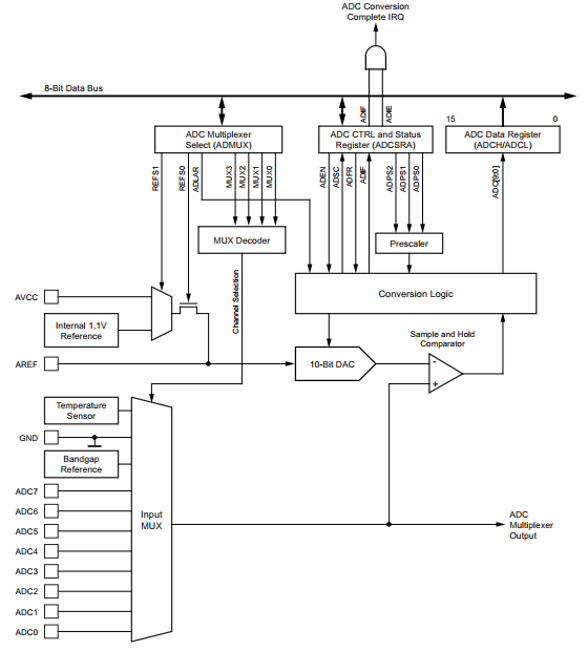
\includegraphics[width=0.8\textwidth]{ADC_sd.png}
	\caption[Sơ đồ khối ADC trên ATmega328p]{Sơ đồ khối ADC trên ATmega328p}
	\label{fig:Sơ đồ khối ADC trên ATmega328p}
\end{figure}

\begin{figure}[h!]
	\centering
	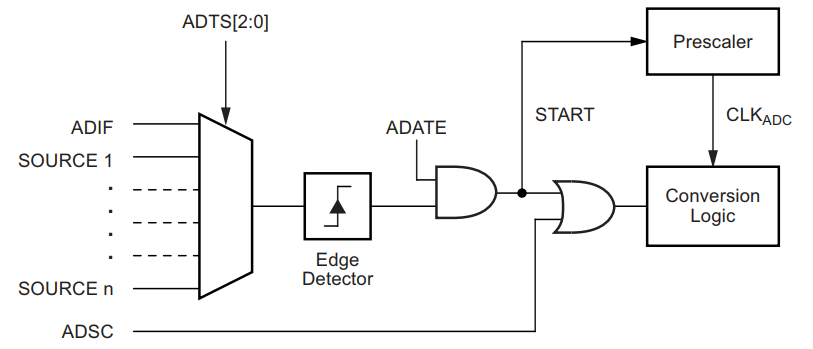
\includegraphics[width=0.8\textwidth]{ADC_hd.png}
	\caption[Hoạt động của khối ADC]{Hoạt động của khối ADC}
	\label{fig:Hoạt động của khối ADC}
\end{figure}

ADTS (ADC Trigger Select): Chọn nguồn đầu vào cho bộ ADC

ADSC (ADC Start Conversion): Bắt đầu chuyển đổi

SOURCE: Nguồn đầu vào analog, ADC0 đến ADC5, tương ứng với PC0 đến PC5

ADATE (ADC Auto Trigger Enable): Tự động chuyển đổi

ADC cần clock trong tầm 50kH tới 200 kHz để đảm bảo độ phân giải tối đa 10 bit.
Trong trường hợp không yêu cầu độ phân giải cao, cần tăng tốc độ lấy mẫu, ADC clock có thể được cấu hình cao hơn 200 kHz.

Việc thay đổi tốc độ ADC clock dựa trên các bit ADPS[2:0] trên thanh ghi ADCSRA.

Thời gian cho 1 lần chuyển đổi thường là 13 ADC clock. Ngoại trừ lần chuyển đổi đầu tiên cần 25 ADC clock.
 
Một số thanh ghi quản lý ADC:
 
\begin{itemize}
	
	\item Thanh ghi ADMUX (ADC multiplexer Selection)
	Là thanh ghi lựa chọn điện áp tham chiếu, căn lề thanh ghi kết quả và lựa chọn kênh đầu vào cho ADC.
	
	\item Thanh ghi ADCSRA (ADC Control and Status Register A)
	Cấu hình và lựa chọn tốc độ lấy mẫu.
	
	\item Thanh ghi ADCSRB (ADC Control and Status Register B)
	Lựa chọn nguồn kích hoạt chế độ lấy mẫu tự động (Auto Conversion).
	
	\item Thanh ghi DIDR0 (Digital Input Disable)
	Loại bỏ đầu vào số cho các Input.
	
	\item Thanh ghi ADCL và ADCH (ADC Data Register)
	Thanh ghi chứa kết quả của quá trình chuyển đổi.
	
\end{itemize}

Giá trị của ADC nằm trong khoảng từ 0 - 1023 sau đó được chuyển về từ 0 - 360 ứng với 360 độ của động cơ. Giá trị ADC này sau đó được chuyển đổi tiếp thành giá trị của đĩa encoder tương ứng với góc quay của động cơ.

\subsubsection{Giao tiếp TWI}

Nhằm thuận tiện cho quá trình theo dõi hoạt động của hệ thống, mô hình sử dụng màn hình LCD1602 được gắn module I2C PCF8574, giao tiếp TWI với vi điều khiển. Các thống số như SP, PV hay giá trị góc quay sẽ được hiển thị lên LCD.

Chuẩn giao tiếp TWI được nghiên cứu và phát triển bởi Atmel, thực chất chính là chuẩn I2C của Philips Semiconductor với cái tên khác. Đây là giao tiếp sử dụng 2 dây kết nối là SCK (Serial Clock) và SDA (Serial Data), là chuẩn giao tiếp không đồng bộ và bán song công (half-duplex). Hai dây SCK và SDA cần điện trở kéo lên (Pull up resistor). Chế độ làm việc theo mô hình Multi-Master với cơ chế phân xử xung đột thiết bị chủ. Tốc độ clock cao nhất đạt 400 kHz. Slave được định địa chỉ 7 bit bằng lập trình, hỗ trợ General Call.

Các chế độ là việc của giao tiếp TWI:
\begin{itemize}
	
	\item Master: Là thiết bị khởi tạo và kết thúc giao tiếp. Master sẽ tạo ra xung clock trên đường SCL. Master sẽ gửi địa chỉ yêu cầu kết nối với slave trên bus.
	\item Slave: Thiết bị được master gửi địa chỉ yêu cầu kết nối trên bus.
	\item Transmitter (Bộ truyền): Là thiết bị gửi dữ liệu lên trên bus.
	\item Receiver (Bộ nhận): Là thiết bị đọc dữ liệu trên bus.
	\item Như vậy sẽ có 4 chế độ cho thiết bị TWI là Master-transmit, Master-receive, Slave-transmit và Slave-receive.

\end{itemize}



\subsubsection{Giao tiếp USART}
USART (Universal Synchronous and Asynchronous serial Receiver and Transmitter): Là bộ truyền nhận thông tin nối tiếp, dữ liệu được truyền theo từng bit liên tục với nhau.

Có 2 chế độ: Đồng bộ và không đồng bộ

\begin{itemize}
	
	\item Master: Không đồng bộ: Hai bên thu và nhận có nguồn clock riêng, dữ liệu được gửi theo từng byte (thêm bit start, stop và parity). Thường dung trong truyền dữ liệu giữa các thiết bị khác nhau.
	\item Slave: Đồng bộ: Hai bên thu và nhận sử dụng chung 1 nguồn clock, dữ liệu được gửi liên tục không cần bit start, stop và parity. Thường dung trong truyền dữ liệu on board.
	
\end{itemize}

Giao thức hoạt động ở chế độ song công (Full duplex), hỗ trợ khung truyền tin 5,6,7,8 hoặc 9 bit dữ liệu, 1 hoặc 2 bit dừng (stop bit), hỗ trợ kiểm tra lỗi (Check parity). Có 3 ngắt: Ngắt TX, ngắt TX data Register empty và ngắt RX.

Sơ đồ khối USART:

\begin{figure}[h!]
	\centering
	\includegraphics[width=0.8\textwidth]{USART.png}
	\caption[Sơ đồ khối USART]{Sơ đồ khối USART}
	\label{fig:Sơ đồ khối USART}
\end{figure}

Chia làm 3 khối chính: Clock Generator, Transmitter và Receiver.

Chân XCK (PD4) chỉ dung trong chế độ đồng bộ.

Chân TX (PD1) là chân truyền tín hiệu (Transmit).

Chân RX (PD0) là chân nhận tín hiệu (Receiver).

Giao tiếp USART được sử dụng nhằm phục vụ xử lý số liệu và vẽ đồ thị hoạt động của hệ thống.


\subsection{Ảnh mô hình}

Vỏ hộp và các linh kiện được thiết kế và in 3D. Mô hình điều khiển vị trí góc động cơ. Có thể thay đổi giá trị SP bằng cách vặn chiết áp. Giá trị SP sau đó được hiển thị lên màn hình LCD1602, đồng thời động cơ cũng quay một góc có độ lớn đúng bằng độ lớn của giá trị SP. Mỗi vạch trên đĩa ứng với 10 độ, mũi trên trên trục động cơ sẽ giúp xác định góc quay của động cơ. 

\begin{figure}[h!]
	\centering
	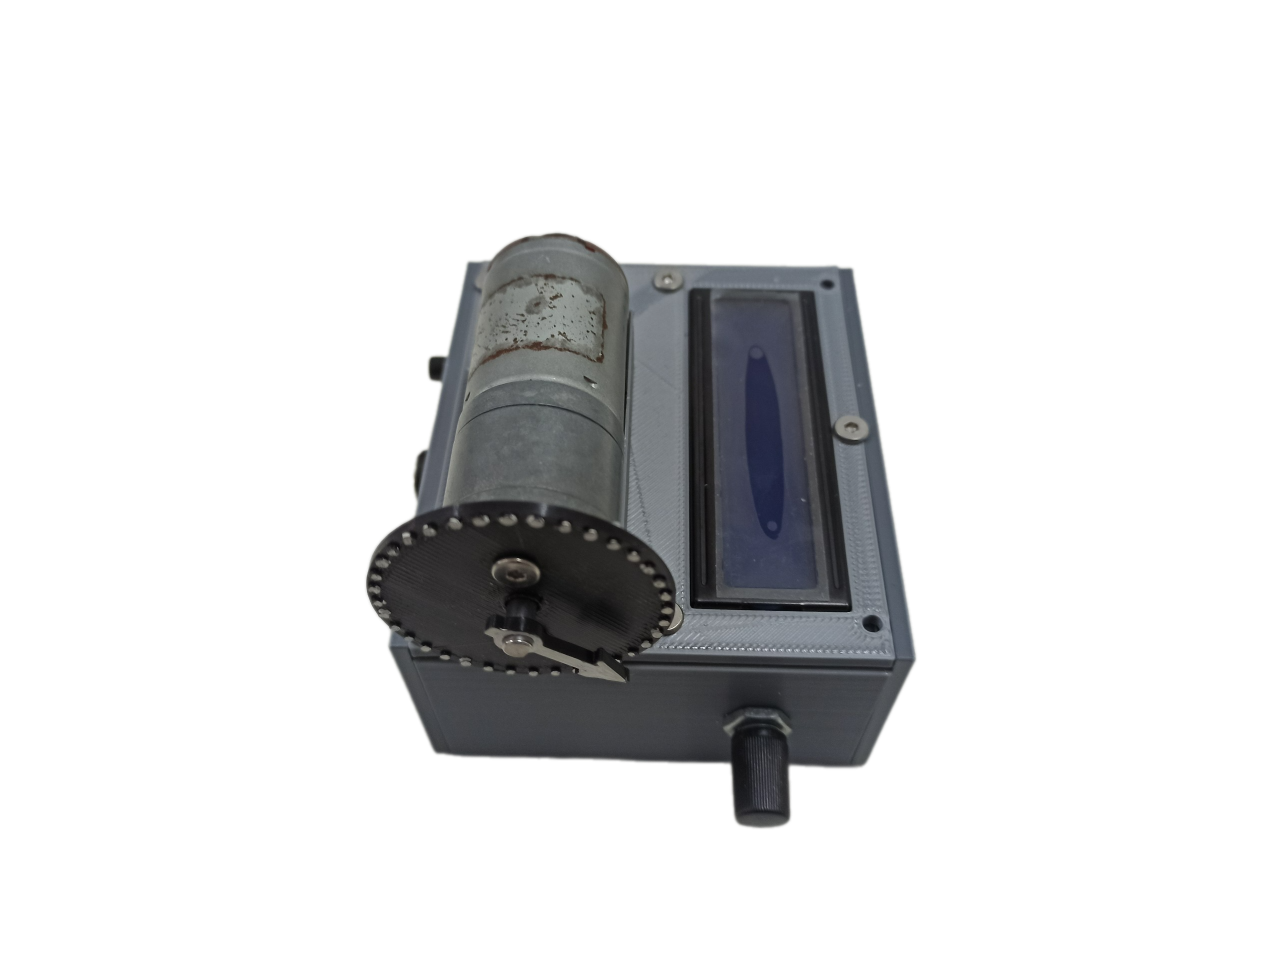
\includegraphics[width=0.8\textwidth]{dc_enc.jpg}
	\caption[Mô mình điều khiển vị trí góc quay động cơ]{Mô mình điều khiển vị trí góc quay động cơ}
	\label{fig:Mô mình điều khiển vị trí góc quay động cơ}
\end{figure}
\newpage
\subsection{Sơ đồ linh kiện}

Mô hình được sử dụng một nguồn 12V cung cấp nguồn nuôi cho động cơ, hai chân ENA và ENB của L298N cần được nối với chân xung của vi điều khiển, chân GND cần được nối chung cho toàn mạch. Chi tiết sơ đồ chân nối được ghi ở phần phụ lục \ref{AppendixB}

\begin{figure}[h!]
	\centering
	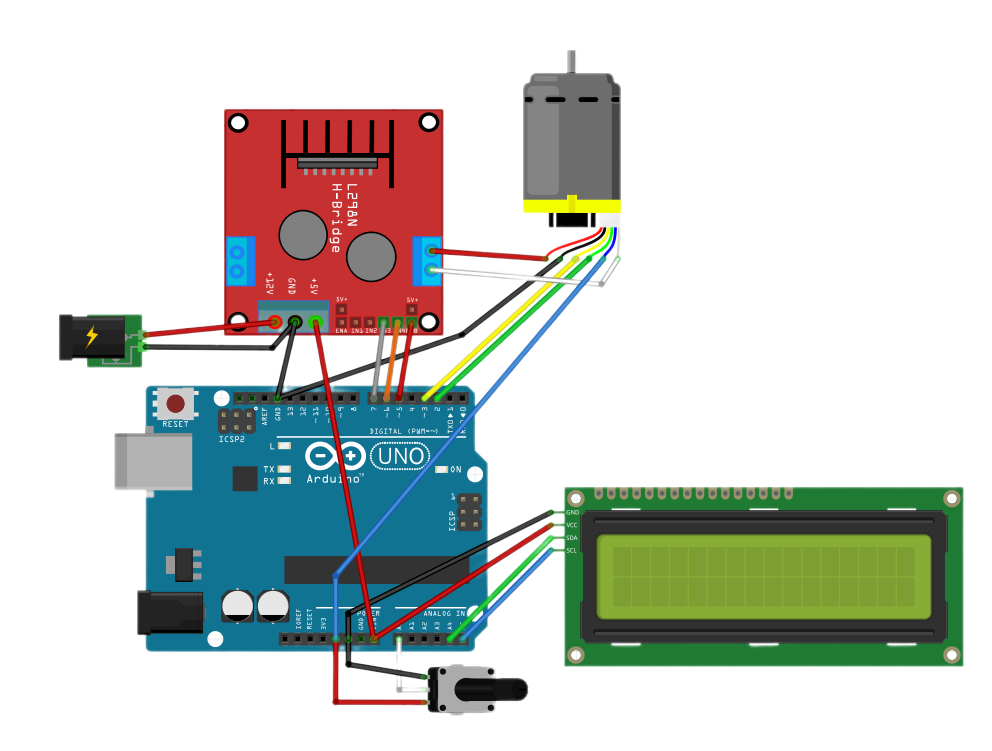
\includegraphics[width=0.8\textwidth]{sche_dc-enc.png}
	\caption[Sơ đồ chân mô mình điều khiển vị trí góc quay động cơ]{Sơ đồ chân mô mình điều khiển vị trí góc quay động cơ}
	\label{fig:Sơ đồ chân mô mình điều khiển vị trí góc quay động cơ}
\end{figure}
\newpage
\subsection{Thiết kế mạch in}

Mạch in của mô hình được thiết kế bằng phần mềm Altium.

\begin{figure}[h!]
	\centering
	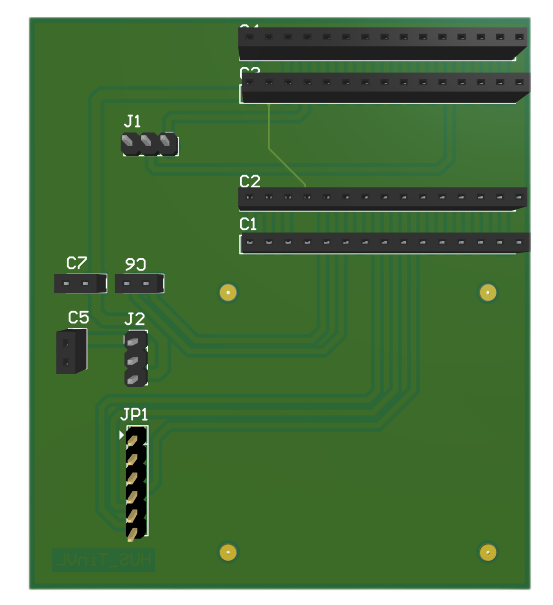
\includegraphics[width=0.8\textwidth]{pcb_dc-enco.png}
	\caption[Thiết kế mạch in mô mình điều khiển vị trí góc quay động cơ DC Encoder]{Thiết kế mạch in mô mình điều khiển vị trí góc quay động cơ DC Encoder}
	\label{fig:Thiết kế mạch in mô mình điều khiển vị trí góc quay động cơ DC Encoder}
\end{figure}
\newpage
\subsection{Thiết kế vỏ hộp}
 Vỏ hộp của mô hình được thiết kế bằng phần mềm Fusion360 sau đó được in 3D.
 
 \begin{figure}[h!]
 	\centering
 	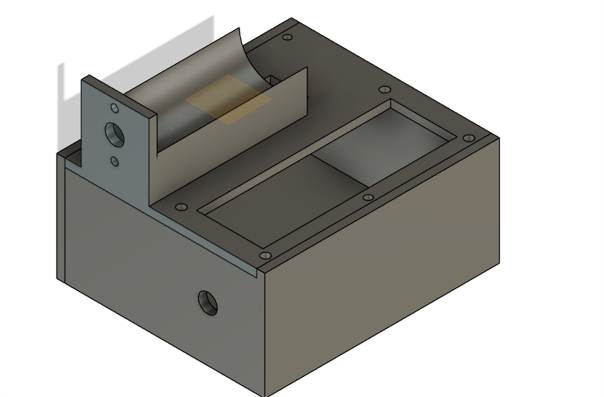
\includegraphics[width=0.8\textwidth]{hop.png}
 	\caption[Vỏ hộp của mô hình được vẽ 3D]{Vỏ hộp của mô hình được vẽ 3D}
 	\label{fig:Vỏ hộp của mô hình được vẽ 3D}
 \end{figure}


\subsection{Phương pháp tìm $K_p$, $K_i$, $K_d$}
\subsubsection{Với bộ điều khiển PID}
Sử dụng phương pháp Ziegler-Nichols 2 để tìm độ lợi cho hệ thống, cùng với đó là hiệu chỉnh thủ công và tiến hành khảo sát để tìm ra ba hằng số độ lợi cho mô hình. Ở mô hình này, ba hằng số độ lợi $K_p$, $K_i$  và $K_d$ lần lượt là 6,75 ; 12,14 và 0,22.

\subsubsection{Với bộ điều khiển PD}
Bằng cách lược bỏ khâu tích phân trong bộ điều khiển PID, bộ điều khiển PD được xây dựng cho mô hình điều khiển vị trí động cơ DC Encoder. Tiến hành tìm thông số $K_p$, $K_d$ cho hệ thống. Ở đây, hai giá trị $K_p$ và $K_d$ lần lượt được xác định bằng 6,7 và 0,2.
\newpage
\subsection{Kết quả}
Hệ thống hoạt động ổn định với các giá trị góc được đặt ra. Khi ta thay đổi setpoint bằng cách vặn chiết áp, giá trị này sẽ được hiển thị lên màn hình LCD, đồng thời động cơ cũng quay một góc bằng giá trị setpoint. Cụ thể trong từng bộ điều khiển PD và PID sẽ cho các kết quả như sau.

\subsubsection{Với bộ điều khiển PD}

Khảo sát hoạt động của hệ thống với bộ điều khiển PD cho thấy hệ thống hoạt động tương đối chính xác, phản hồi nhanh. 

 \begin{figure}[h!]
	\centering
	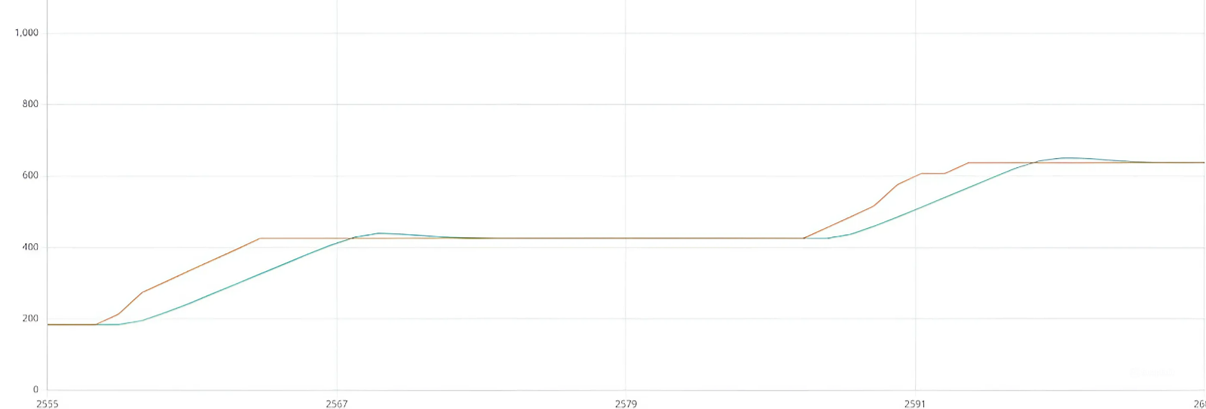
\includegraphics[width=0.9\textwidth]{pd1.png}
	\caption[Hoạt động của hệ thống với bộ điều khiển PD (1)]{Hoạt động của hệ thống với bộ điều khiển PD (1)}
	\label{fig:Hoạt động của hệ thống với bộ điều khiển PD (1)}
\end{figure}

Tuy nhiên trong một số trường hợp giá trị PV khác giá trị SP thì hệ thống không thể tính toán để điều khiển giá trị PV = SP do bộ điều khiển không có thành phần tích phân. 

 \begin{figure}[h!]
	\centering
	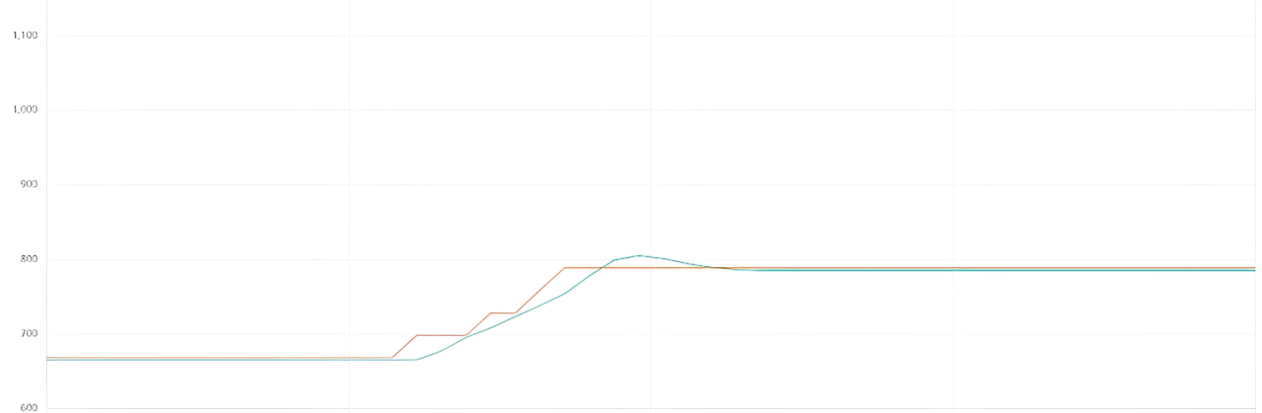
\includegraphics[width=0.9\textwidth]{pd2.png}
	\caption[Hoạt động của hệ thống với bộ điều khiển PD (2)]{Hoạt động của hệ thống với bộ điều khiển PD (2)}
	\label{fig:Hoạt động của hệ thống với bộ điều khiển PD (2)}
\end{figure}

Đổi lại hệ thống hoạt động với độ ổn định cao, không xảy ra hiện tượng dao động.
\newpage
\subsubsection{Với bộ điều khiển PID}

Với bộ điều khiển PID, hệ thống cho thấy độ chính xác cao trong quá trình hoạt động.

 \begin{figure}[h!]
	\centering
	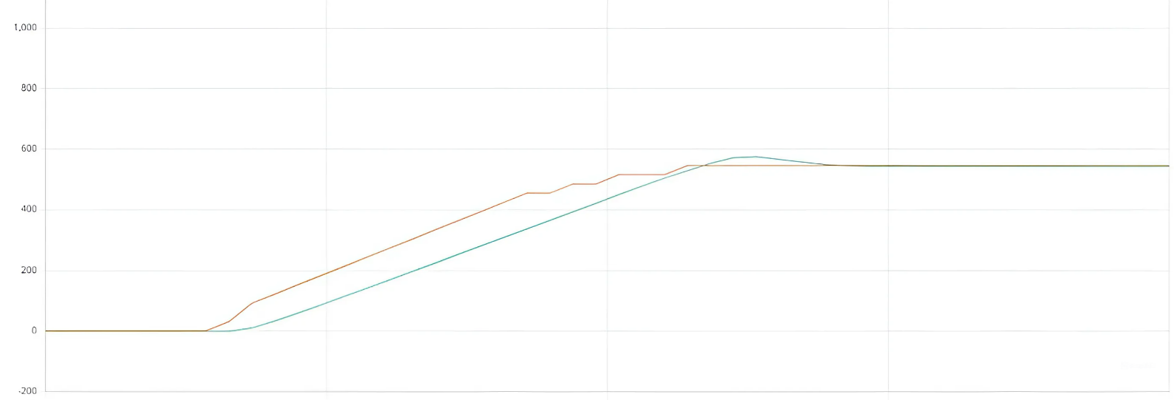
\includegraphics[width=0.9\textwidth]{pid1.png}
	\caption[Hoạt động của hệ thống với bộ điều khiển PID (1)]{Hoạt động của hệ thống với bộ điều khiển PID (1)}
	\label{fig:Hoạt động của hệ thống với bộ điều khiển PID (1)}
\end{figure}

Trong trường hợp giá trị PV chưa bằng SP, thành phần tích phân sẽ tích lũy giá trị sai số và tiếp tục điều khiển động cơ sao cho hai giá trị này bằng nhau. Điều này sẽ giúp cho hệ thống hoạt động với độ chính xác cao.

Tuy vậy, việc tích lũy tích phân sai số cũng sẽ khiến hệ thống mất đi tính ổn định, trong một số trường hợp động cơ còn xảy ra hiện tượng dao động. Nguyên nhân là do ba hằng số độ lợi chưa hoàn toàn tối ưu với hệ thống.

 \begin{figure}[h!]
	\centering
	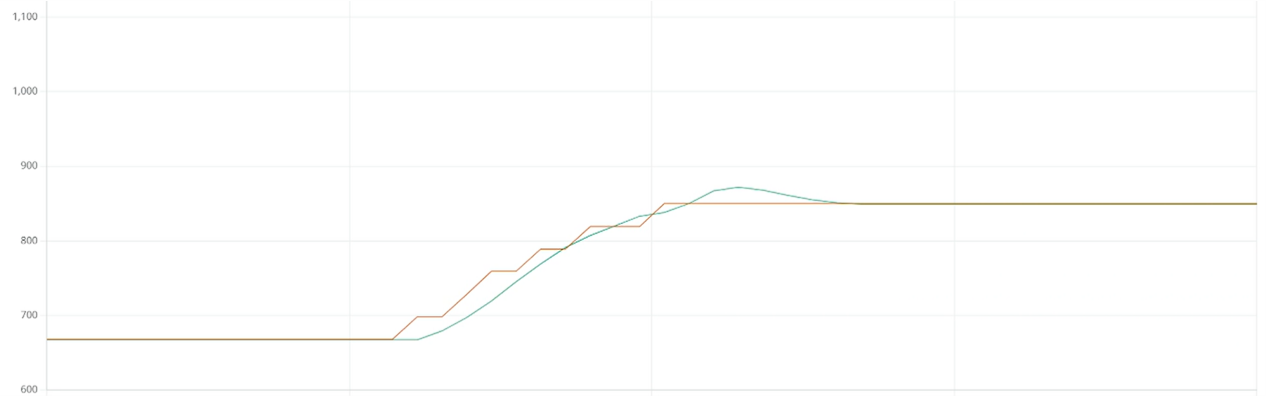
\includegraphics[width=0.9\textwidth]{pid2.png}
	\caption[Hoạt động của hệ thống với bộ điều khiển PID (2)]{Hoạt động của hệ thống với bộ điều khiển PID (2)}
	\label{fig:Hoạt động của hệ thống với bộ điều khiển PID (2)}
\end{figure}
 
% Chương 3

\chapter{KẾT QUẢ} % Tên của chương

\label{Chapter3} % Để trích dẫn chương này ở chỗ nào đó trong bài, hãy sử dụng lệnh \ref{Chapter3} 

%----------------------------------------------------------------------------------------

% Định nghĩa một số lệnh cần thiết để điều chỉnh định dạng cho một số nội dung nhất định trong bài

%\newcommand{\keyword}[1]{\textbf{#1}}
%\newcommand{\tabhead}[1]{\textbf{#1}}
%\newcommand{\code}[1]{\texttt{#1}}
%\newcommand{\file}[1]{\texttt{\bfseries#1}}
%\newcommand{\option}[1]{\texttt{\itshape#1}}

%----------------------------------------------------------------------------------------

\section{Kết luận chung}
Sau thời gian tìm hiểu về lý thuyết của bộ điều khiển PID cùng với ứng dụng của bộ điều khiển này vào mô hình điều khiển vị trí góc quay động cơ DC Encoder, báo cáo này đã đạt được một số kết quả. 

\subsection{Bộ điều khiển PID}
\begin{itemize}
	\item Lịch sử hình thành, cơ cấu hoạt động của thuật toán điều khiển PID.	
	\item Hiểu rõ về bộ điều khiển PID dạng song song, các thành phần và vai trò của chúng trong bộ điều khiển.
	\item Tìm hiểu về một số phương pháp tìm độ lợi $K_p$ $K_i$ $K_d$ giúp tối ưu độ ổn định của các hệ thống trong quá trình hoạt động.
	\item Tính hiệu quả, độ tin cậy của bộ điều khiển PID, các ứng dụng của bộ điều khiển này trong đời sống con người.
	\item Xây dựng một số mô hình sử dụng thuật toán PID nhằm chứng minh cơ cấu hoạt động, tính hiệu quả của thuật toán.
\end{itemize}

\subsection{Các mô hình thực tế sử dụng thuật toán PID}
Mô hình sử dụng thuật toán PID đều hoạt động một cách ổn định. Phản hồi của hệ thống nhanh khi bị tác động bởi các yếu tố khách quan. Bộ điều khiển này đã chứng minh được tính ổn định và tối ưu của nó trong việc điều khiển một số hệ thống. Các hệ thống trong quá trình hoạt động đều đạt được tính ổn định cao, đồng thời cho thấy tính đơn giản và hiệu quả của thuật toán PID.
\newpage
\subsection{Các chức năng của vi điều khiển}
\begin{itemize}
	\item Học được kỹ năng đọc datasheet của linh kiện cần sử dụng.
	\item Hiểu về lập trình nhúng AVR, chức năng của các thanh ghi trong vi điều khiển ATmega328p.
	\item Thành thạo trong việc sử dụng các chức năng khác của Timer như: tạo xung PWM. Sử dụng ngắt để xử lý các tình huống trong lập trình vi điều khiển.
	\item Hiểu rõ và ứng dụng các giao thức được sử dụng phổ biến như TWI, USART...
	\item Học được cách viết chương trình nhằm tối ưu hóa hoạt động của vi điều khiển.
	  
\end{itemize}
\section{Một số vấn đề còn tồn tại của đề tài}
Cùng với các kết quả đạt được, đề tài này còn tồn tại một số vấn đề. Mô hình và bộ điều khiển PID còn ở dạng đơn giản. Chưa mô hình hóa được hệ thống tổng thể và phương trình toán học cụ thể cho từng mô hình. Ngoài ra, chưa tìm hiểu và khảo sát các phương pháp tìm độ lợi khác.
 
\section{Hướng phát triển của đề tài}
Bên cạnh kết quả thu được và một số hạn chế, đề tài này vẫn có thể được phát triển hơn nữa trong tương lai. Nâng cấp các cảm biến đang sử dụng trong các mô hình, sử dụng các chip xử lí tốc độ cao nhằm tối ưu hơn nữa quá trình tính toán và các hệ thống. Tìm hiểu về một số phương thức truyền dữ liệu không dây để có thể xử lý hệ thống. Nghiên cứu sâu hơn về bộ điều khiển PID, các dạng khác của bộ điều khiển này như: Dạng Laplace, dạng nối tiếp/ tương hỗ... Có thể biễu diễn các mô hình dưới dạng phương trình toán học. Sử dụng thuật toán PID trong các mô hình lớn hơn như: điều khiển lò nhiệt, chế tạo drone, xe segway...



%\include{Chapters/Chapter4} 
%\include{Chapters/Chapter5} 

%----------------------------------------------------------------------------------------
%	(KHÔNG CHỈNH SỬA PHẦN NÀY)
%
%	PHẦN 13: TÀI LIỆU THAM KHẢO
%----------------------------------------------------------------------------------------

\begin{spacing}{1.15}
	\printbibliography[heading=bibintoc, title=Tài liệu tham khảo] % In ra tài liệu tham khảo
	\nocite{dung}
	\nocite{nam}
	\nocite{aastrom2001future}
	\nocite{aastrom2002control}
	\nocite{borase2021review}
	\nocite{kiong1999advances}
	\nocite{lin2000self}
	\nocite{vilanova2012pid}
	\nocite{bao1}
	\nocite{bao2}
	\nocite{bao3}
	\nocite{ang2005pid}


\end{spacing}

%----------------------------------------------------------------------------------------
%	PHẦN 14: PHỤ LỤC (THESIS CONTENT - APPENDICES)
%----------------------------------------------------------------------------------------

\appendix % Nói với LaTeX rằng những chương về sau được tính là phụ lục

% Hãy thêm những phụ lục (appendix) của khóa luận/tiểu luận vào thư mục Appendices
% Hãy bỏ chú thích những dòng nếu bạn đã bổ sung những phụ lục vào

% Phụ lục A

\chapter{Các chương trình của đề tài} % Tên của phụ lục

\label{AppendixA} % Để trích dẫn chương này ở chỗ nào đó trong bài, hãy sử dụng lệnh \ref{AppendixA} 

%----------------------------------------------------------------------------------------

\section{Chương trình chính (main.c)}

	\begin{lstlisting}
/*
* GccApplication1.c
*
* Created: 5/23/2024 3:04:35 PM
* Author : letung
*/ 
#define F_CPU 16000000UL
#define deltaT 0.04
#include <avr/io.h>
#include <util/delay.h>
#include <avr/interrupt.h>
#include <stdio.h>
#include <math.h>
#include <stdbool.h>
#include "uart.h"
#include "ADCLib.h"
#include "hd44780pcf8574.h"


char addr = PCF8574_ADDRESS;  //0x27
float ADC_value = 0;
float setpoint = 0;
float pos = 0;

int b;
char str_sp[5];
char str_pv[5]; 
char str_angle[5];

long prevT = 0;
float eprev = 0;
float eintegral = 0;

bool Saturation = false;

// PID parameters
float kp = 6.75;
float ki = 12.14;
//float ki = 0;
float kd = 0.22;

ISR(INT0_vect){
	b = PIND & (1 << PD3); 
	if (b) pos++;
	else pos--; 	
}
void setMotor(int dir, int pwmVal) {
	OCR0B = pwmVal;
	if (dir == 1) {
		PORTD |= (1 << PD7);
		PORTD &= ~(1 << PD6);
	} else if (dir == -1) {
		PORTD &= ~(1 << PD7);
		PORTD |= (1 << PD6);
	} else {
		PORTD &= ~(1 << PD7);
		PORTD &= ~(1 << PD6);
	}
	
}
int main(void)
{
	HD44780_PCF8574_Init(addr);
	HD44780_PCF8574_DisplayClear(addr);
	HD44780_PCF8574_DisplayOn(addr);
	HD44780_PCF8574_DrawString(addr, "Embedded System");
	_delay_ms(1000);
	HD44780_PCF8574_DisplayClear(addr);
	HD44780_PCF8574_PositionXY(addr, 0, 0);
	HD44780_PCF8574_DrawString(addr,"SP:");
	HD44780_PCF8574_PositionXY(addr, 0, 1);
	HD44780_PCF8574_DrawString(addr,"PV:");
	//_delay_ms(100);
	uart_init(9600);
	ADC_init(0);
	
	DDRD |= (1 << PD5) | (1 << PD6) | (1 << PD7);
	TCCR0A |= (1 << WGM00) | (1 << WGM01) | (1 << COM0B1); // Fast PWM, non-inverting mode
	TCCR0B |= (1 << CS00) | (1 << CS01); // Prescaler 64
	
	EICRA=(0<<ISC11) | (0<<ISC10) | (1<<ISC01) | (1<<ISC00);
	EIMSK=(0<<INT1) | (1<<INT0);
	EIFR=(0<<INTF1) | (1<<INTF0);
	sei();
	
	
	
	while (1) 
	{
		
		read_ADC();
		ADC_value = ADCW;
		ADC_value = 10*round(ADC_value*36/1023);
		setpoint = round((11 * 99.3 * ADC_value)/360);
		int e = setpoint - pos;
		float dedt = (e - eprev) / deltaT;
		if (!Saturation) {
			eintegral += (e + eprev) * deltaT / 2;
		}
		// PID calculation
		float u = kp * e + ki * eintegral + kd * dedt;
		
		float pwr = fabs(u);
		if (pwr > 255) {
			pwr = 255;
			Saturation = true;
		} else {
			Saturation = false;
		}
		
		// Motor direction
		int dir;
		if (u < 0) {
			dir = -1;
		} else {
			dir = 1;
		}
		
		// Set motor
		setMotor(dir, pwr);
		
		// Store previous error
		eprev = e;
		
		sprintf(str_angle, "%4.0f",ADC_value);
		sprintf(str_sp, "%4.0f",setpoint);
		sprintf(str_pv, "%4.0f",pos);
		HD44780_PCF8574_PositionXY(addr, 4, 0);
		HD44780_PCF8574_DrawString(addr,str_angle);
		HD44780_PCF8574_PositionXY(addr, 10, 0);
		HD44780_PCF8574_DrawString(addr,str_sp);
		HD44780_PCF8574_PositionXY(addr, 10, 1);
		HD44780_PCF8574_DrawString(addr,str_pv);
		
		
		uart_putstring("Setpoint:");
		uart_putstring(str_sp);
		uart_putstring("   ");
		uart_putstring(" PV:");
		uart_putstring(str_pv);
		uart_putstring("\n");
	}
}



	\end{lstlisting}

\section{Thư viện ADCLib.h}

	\begin{lstlisting}
	
	#include <avr/io.h>
	#include <util/delay.h>
	#include <stdlib.h>
	#include <stdio.h>
	#include <avr/interrupt.h>
	
	
	void ADC_init(unsigned int pin){
		
		ADMUX = 0b01000000 | pin;
		ADCSRA = 0b10000111;
		DIDR0 |= 0x01 << pin;
		_delay_ms(10);
	}
	
	int read_ADC(){
		ADCSRA |= 0b01000000;
		while((ADCSRA & 0b00010000) == 0);
		ADCSRA |= 0b00010000;
		return ADCW;		
	}
	\end{lstlisting}

\section{Thư viện uart.h}

	\begin{lstlisting}
#ifndef _UARTLIB_
#define _UARTLIB_
#define fosc 16000000
#include <avr/io.h>
//#include <avr/interrupt.h>
#include <util/delay.h>
void uart_init(unsigned int BAUDRATE)
{
	//Config BAUD Rate
	unsigned int n = fosc/BAUDRATE/16 - 1;
	UBRR0H = n>>8;
	UBRR0L = n;
	//Config mode and data frame 
	//Asynchronous mode, 8 data bit, 1 stop bit, no Parity
	UCSR0C = 0b00000110;
	//Enable transmiter and receiver, RX interupt
	UCSR0B = 0b10011000;  
	sei();
}
void uart_putchar(unsigned char data)
{
	while (!(UCSR0A & 0b00100000)); //wait for data register empty
	UDR0 = data;
}
void uart_putstring(char *str)
{
	while (*str)
	{
		uart_putchar(*str); 
		//if see the line feed, add carriage return
		if (*str == '\n')
		uart_putchar('\r');
		str++;
	}
}
void uart_put_int(unsigned int value)
{
	unsigned char buf[8];
	int index = 0,i,j;
	j = value;
	do {
		buf[index] = j%10 + 48;//chuyen gia tri sang ki tu
		j = j/10;
		index +=1;    
	} while(j);
	
	for (i = index; i>0; i--)
	uart_putchar(buf[i-1]);
}

#endif 
	\end{lstlisting}

\section{Thư viện TWI.h}

\begin{lstlisting}
	#include <stdio.h>
	#include <avr/io.h>
	
	#ifndef __TWI_H__
	#define __TWI_H__
	
	// define register for TWI communication
	#if defined(__AVR_ATmega16__) || defined(__AVR_ATmega328P__)
	#define TWI_TWAR TWAR // TWI (Slave) Address Register
	#define TWI_TWBR TWBR // TWI Bit Rate Register
	#define TWI_TWDR TWDR // TWI Data Register
	#define TWI_TWCR TWCR // TWI Control Register
	#define TWI_TWSR TWSR // TWI Status Register
	#endif
	
	// TWI status mask
	#define TWI_STATUS                    (TWI_TWSR & 0xF8)
	#define TWI_WRITE                     0
	#define TWI_READ                      1
	
	// TWI CLK frequency
	//  @param TWBR
	//  @param Prescaler
	//    TWPS1 TWPS0  - PRESCALER
	//      0     0    -     1
	//      0     1    -     4
	//      1     0    -    16
	//      1     1    -    64
	#define TWI_FREQ(BIT_RATE, PRESCALER) { TWI_TWBR = BIT_RATE; TWI_TWSR |= (TWI_TWSR & 0x03) | PRESCALER; }
	
	// TWI start condition
	// (1 <<  TWEN) - TWI Enable
	// (1 << TWINT) - TWI Interrupt Flag - must be cleared by set
	// (1 << TWSTA) - TWI Start
	#define TWI_START()                   { TWI_TWCR = (1 << TWEN) | (1 << TWINT) | (1 << TWSTA); }
	
	// TWI MASTER enable with NACK
	// (1 <<  TWEN) - TWI Enable
	// (1 << TWINT) - TWI Interrupt Flag - must be cleared by set
	#define TWI_MSTR_ENABLE_NACK()        { TWI_TWCR = (1 << TWEN) | (1 << TWINT); }
	
	// TWI MASTER enable with ACK
	// (1 <<  TWEN) - TWI Enable
	// (1 << TWINT) - TWI Interrupt Flag - must be cleared by set
	// (1 <<  TWEA) - TWI Master Receiver will return ACK
	#define TWI_MSTR_ENABLE_ACK()         { TWI_TWCR = (1 << TWEN) | (1 << TWINT) | (1 << TWEA); }
	
	// TWI stop condition
	// (1 <<  TWEN) - TWI Enable
	// (1 << TWINT) - TWI Interrupt Flag - must be cleared by set
	// (1 << TWSTO) - TWI Stop
	#define TWI_STOP()                    { TWI_TWCR = (1 << TWEN) | (1 << TWINT) | (1 << TWSTO); }
	
	// TWI test if TWINT Flag is set
	#define TWI_WAIT_TILL_TWINT_IS_SET()  { while (!(TWI_TWCR & (1 << TWINT))); }
	
	// definitions
	#define TWI_STATUS_INIT       0xFF
	#define TWI_SUCCESS              0
	#define TWI_ERROR                1
	#define TWI_ERROR_NONE           0 
	
	// ++++++++++++++++++++++++++++++++++++++++++
	//
	//        M A S T E R   M O D E
	//
	// ++++++++++++++++++++++++++++++++++++++++++  
	// Master Mode - Transmitter / Receiver
	#define TWI_START_ACK         0x08  // A START condition has been transmitted
	#define TWI_REP_START_ACK     0x10  // A repeated START condition has been transmitted
	#define TWI_FLAG_ARB_LOST     0x38  // Arbitration lost in SLA+W or NOT ACK bit
	// Master Transmitter Mode
	#define TWI_MT_SLAW_ACK       0x18  // SLA+W has been transmitted; ACK has been received
	#define TWI_MT_SLAW_NACK      0x20  // SLA+W has been transmitted; NOT ACK has been received
	#define TWI_MT_DATA_ACK       0x28  // Data byte has been transmitted; ACK has been received
	#define TWI_MT_DATA_NACK      0x30  // Data byte has been transmitted; NOT ACK has been received  
	// Master Receiver Mode
	#define TWI_MR_SLAR_ACK       0x40  // SLA+R has been transmitted; ACK has been received
	#define TWI_MR_SLAR_NACK      0x48  // SLA+R has been transmitted; NOT ACK has been received
	#define TWI_MR_DATA_ACK       0x50  // Data byte has been received; ACK has been received
	#define TWI_MR_DATA_NACK      0x58  // Data byte has been received; NOT ACK has been received
	
	// ++++++++++++++++++++++++++++++++++++++++++
	//
	//         S L A V E   M O D E
	//
	// ++++++++++++++++++++++++++++++++++++++++++
	// Slave Receiver Mode
	#define TWI_SR_SLAW_ACK       0x60  // Own Slave address has been received; ACK returned
	#define TWI_SR_ALMOA_ACK      0x68  // Arbitration Lost in SLA+R/W as Master; Own Slave address has been received; ACK returned
	#define TWI_SR_GCALL_ACK      0x70  // General call address has been received; ACK returned
	#define TWI_SR_ALMGA_ACK      0x78  // Arbitration lost in SLA+R/W as Master; General call address has been received; ACK returned  
	#define TWI_SR_OA_DATA_ACK    0x80  // Previously addressed with own SLA+W; data has been received; ACK returned
	#define TWI_SR_OA_DATA_NACK   0x88  // Previously addressed with own SLA+W; data has been received; NOT ACK returned
	#define TWI_SR_GC_DATA_ACK    0x90  // Previously addressed with general call; data has been received; ACK returned
	#define TWI_SR_GC_DATA_NACK   0x98  // Previously addressed with general call; data has been received; NOT ACK returned
	#define TWI_SR_STOP_RSTART    0xA0  // A STOP condition or repeated START condition has been received while still addressed as Slave
	// Slave Transmitter Mode
	#define TWI_ST_OA_ACK         0xA8  // Own SLA+R has been received; ACK has been returned
	#define TWI_ST_ALMOA_ACK      0xB0  // Arbitration lost in SLA+R/W as Master; own SLA+R has been received; ACK has been received
	#define TWI_ST_DATA_ACK       0xB8  // Data byte in TWDR has been transmitted; ACK has been received
	#define TWI_ST_DATA_NACK      0xC0  // Data byte in TWDR has been transmitted; NOT ACK has been received
	#define TWI_ST_DATA_LOST_ACK  0xC8  // Last data byte in TWDR has been transmitted (TWEA = '0'); ACK has been received
	
	 
	extern char _twi_error_stat;
	

	void TWI_Init (void);
	

	void TWI_MT_Start (void);
	

	void TWI_Transmit_SLAW (char);
	

	void TWI_Transmit_SLAR (char);
	

	void TWI_Transmit_Byte (char);
	

	char TWI_Receive_Byte (void);
	

	void TWI_Stop (void);

	void TWI_Error (char, char);
	
	#endif
	
\end{lstlisting}


\section{Thư viện TWI.c }

\begin{lstlisting}

	#include "twi.h"
	
	/* @var error status */  
	char _twi_error_stat = TWI_ERROR_NONE;
	
	/**
	* @desc    TWI init - initialize frequency
	*
	* @param   void
	*
	* @return  void
	*/
	void TWI_Init(void)
	{
		// +++++++++++++++++++++++++++++++++++++++++++++
		// Calculation fclk:
		//
		// fclk = (fcpu)/(16+2*TWBR*4^Prescaler)
		// --------------------------------------------- 
		// Calculation TWBR:
		// 
		// TWBR = {(fcpu/fclk) - 16 } / (2*4^Prescaler)
		// +++++++++++++++++++++++++++++++++++++++++++++
		// @16MHz
		// @param1 value of TWBR, 
		//    fclk = 400 kHz; TWBR = 3
		//    fclk = 200 kHz; TWBR = 8
		//    fclk = 100 kHz; TWBR = 18
		// @8MHz
		// @param1 value of TWBR, 
		//    fclk = 200 kHz; TWBR = 3
		//    fclk = 100 kHz; TWBR = 8
		// @param2 value of Prescaler = 1
		TWI_FREQ(8, 1);
	}
	
	/**
	* @desc    TWI MT Start
	*
	* @param   void
	*
	* @return  void
	*/
	void TWI_MT_Start(void)
	{ 
		// init status
		char status = TWI_STATUS_INIT;
		// START
		// ----------------------------------------------
		// request for bus
		TWI_START();
		// wait till flag set
		TWI_WAIT_TILL_TWINT_IS_SET();
		// status read
		status = TWI_STATUS;
		// test if start or repeated start acknowledged
		if ((status != TWI_START_ACK) && (status != TWI_REP_START_ACK)) {
			// error status
			TWI_Error(status, TWI_START_ACK);
		}
	}
	
	/**
	* @desc    TWI Send address + write
	*
	* @param   char
	*
	* @return  void
	*/
	void TWI_Transmit_SLAW(char address)
	{
		// init status
		char status = TWI_STATUS_INIT;
		// SLA+W
		// ----------------------------------------------
		TWI_TWDR = (address << 1);
		// enable
		TWI_MSTR_ENABLE_ACK();
		// wait till flag set
		TWI_WAIT_TILL_TWINT_IS_SET();
		// status read
		status = TWI_STATUS;
		// find
		if (status != TWI_MT_SLAW_ACK) {
			// error status
			TWI_Error(status, TWI_MT_SLAW_ACK);
		}
	}
	
	/**
	* @desc    TWI Send address + read
	*
	* @param   char
	*
	* @return  void
	*/
	void TWI_Transmit_SLAR(char address)
	{
		// init status
		char status = TWI_STATUS_INIT;
		// SLA+R
		// ----------------------------------------------
		TWI_TWDR = (address << 1) | TWI_READ;
		// enable
		TWI_MSTR_ENABLE_ACK();
		// wait till flag set
		TWI_WAIT_TILL_TWINT_IS_SET();
		// status read
		status = TWI_STATUS;
		// find
		if (status != TWI_MR_SLAR_ACK) {
			// error status
			TWI_Error(status, TWI_MR_SLAR_ACK);
		}
	}
	
	/**
	* @desc    TWI Transmit data
	*
	* @param   char
	*
	* @return  void
	*/
	void TWI_Transmit_Byte(char data)
	{
		// init status
		char status = TWI_STATUS_INIT;
		// DATA SEND
		// ----------------------------------------------
		TWI_TWDR = data;
		// enable
		TWI_MSTR_ENABLE_ACK();
		// wait till flag set
		TWI_WAIT_TILL_TWINT_IS_SET();
		// status read
		status = TWI_STATUS;
		// send with success
		if (status != TWI_MT_DATA_ACK) {
			// error status
			TWI_Error(status, TWI_MT_DATA_ACK);
		}
	}
	
	/**
	* @desc    TWI Receive 1 byte
	*
	* @param   void
	*
	* @return  char
	*/
	char TWI_Receive_Byte(void)
	{
		// init status
		char status = TWI_STATUS_INIT;
		// DATA RECEIVE
		// ----------------------------------------------
		// enable with NACK
		TWI_MSTR_ENABLE_NACK();
		// wait till flag set
		TWI_WAIT_TILL_TWINT_IS_SET();
		// status read
		status = TWI_STATUS;
		// send with success
		if (status != TWI_MR_DATA_NACK) {
			// error status
			TWI_Error(status, TWI_MR_DATA_NACK);
		}
		// received data
		return TWI_TWDR;
	}
	
	
	void TWI_Stop(void)
	{
		// End TWI
		// -------------------------------------------------
		// send stop sequence
		TWI_STOP();
		// wait for TWINT flag is set
		//  TWI_WAIT_TILL_TWINT_IS_SET();
	}
	
	
	void TWI_Error(char status, char expected)
	{ 
		
	}



\end{lstlisting}


\section{Thư viện LCD I2C - hd44780pcf8574.h }

\begin{lstlisting}
	
	#ifndef __HD44780PCF8574_H__
	#define __HD44780PCF8574_H__
	
	#include <avr/io.h>
	#include <avr/pgmspace.h>
	
	#define PCF8574_SUCCESS         0
	#define PCF8574_ERROR           1
	#define PCF8574_ADDRESS      0x27
	
	
	#define PCF8574_PIN_RS       0x01
	#define PCF8574_PIN_RW       0x02
	#define PCF8574_PIN_E        0x04
	#define PCF8574_PIN_P3       0x08
	#define PCF8574_PIN_DB4      0x10
	#define PCF8574_PIN_DB5      0x20
	#define PCF8574_PIN_DB6      0x40
	#define PCF8574_PIN_DB7      0x80
	
	#define HD44780_BUSY_FLAG    HD44780_DB7
	#define HD44780_INIT_SEQ     0x30
	#define HD44780_DISP_CLEAR   0x01
	#define HD44780_DISP_OFF     0x08
	#define HD44780_DISP_ON      0x0C
	#define HD44780_CURSOR_ON    0x0E
	#define HD44780_CURSOR_BLINK 0x0F
	#define HD44780_RETURN_HOME  0x02 
	#define HD44780_ENTRY_MODE   0x06
	#define HD44780_4BIT_MODE    0x20
	#define HD44780_8BIT_MODE    0x30
	#define HD44780_2_ROWS       0x08
	#define HD44780_FONT_5x8     0x00
	#define HD44780_FONT_5x10    0x04
	#define HD44780_POSITION     0x80
	
	#define HD44780_SHIFT        0x10
	#define HD44780_CURSOR       0x00
	#define HD44780_DISPLAY      0x08
	#define HD44780_LEFT         0x00
	#define HD44780_RIGHT        0x04
	
	#define HD44780_ROWS         2
	#define HD44780_COLS         16
	
	#define HD44780_ROW1_START   0x00
	#define HD44780_ROW1_END     HD44780_COLS
	#define HD44780_ROW2_START   0x40
	#define HD44780_ROW2_END     HD44780_COLS
	
	// set bit
	#define SETBIT(REG, BIT) { REG |= (1 << BIT); }
	// clear bit
	#define CLRBIT(REG, BIT) { REG &= ~(1 << BIT); }
	// set port / pin if bit is set
	#define SET_IF_BIT_IS_SET(REG, PORT, DATA, BIT) { if((DATA & BIT) > 0) { SETBIT(REG, PORT); } }
	
	char HD44780_PCF8574_Init (char);
	
	void HD44780_PCF8574_E_pulse (char);
	
	void HD44780_PCF8574_SendInstruction (char, char);
	
	void HD44780_PCF8574_SendData (char, char);
	
	void HD44780_PCF8574_CheckBF (char);
	
	void HD44780_PCF8574_Send_4bits_M4b_I (char);
	
	void HD44780_PCF8574_Send_8bits_M4b_I (char, char, char);
	
	void HD44780_PCF8574_DisplayClear (char);
	
	void HD44780_PCF8574_DisplayOn (char);
	
	void HD44780_PCF8574_CursorOn (char);
	
	void HD44780_PCF8574_CursorBlink (char);

	void HD44780_PCF8574_DrawChar (char, char);
	
	void HD44780_PCF8574_DrawString (char, char *);
	
	char HD44780_PCF8574_PositionXY (char, char, char);
	
	char HD44780_PCF8574_Shift (char, char, char);
	
	#endif
	
	
\end{lstlisting}

\section{Thư viện LCD I2C - hd44780pcf8574.c}

\begin{lstlisting}
	#include <stdio.h>
	#include <util/delay.h>
	#include <avr/io.h>
	#include "twi.h"
	#include "hd44780pcf8574.h"
	
	// +---------------------------+
	// |         Power on          |
	// | Wait for more than 15 ms  |   // 15 ms wait
	// | after VCC rises to 4.5 V  |
	// +---------------------------+
	//              |
	// +---------------------------+ 
	// |  RS R/W DB7 DB6 DB5 DB4   |   
	// |   0   0   0   0   1   1   |   // Initial sequence 0x30
	// | Wait for more than 4.1 ms |   // 4.1 ms us writing DATA into DDRAM or CGRAM
	// +---------------------------+
	//              |
	// +---------------------------+
	// |  RS R/W DB7 DB6 DB5 DB4   |   
	// |   0   0   0   0   1   1   |   // Initial sequence 0x30
	// | Wait for more than 0.1 ms |   // 100 us writing DATA into DDRAM or CGRAM
	// +---------------------------+
	//              |
	// +---------------------------+
	// |  RS R/W DB7 DB6 DB5 DB4   |   // Initial sequence 0x30
	// |   0   0   0   0   1   1   |   // 37 us writing DATA into DDRAM or CGRAM 4 us tadd - time after busy flag disapeared
	// | Wait for more than 45 us  |   // 37 us + 4 us = 41 us * (270/250) = 45us
	// +---------------------------+  
	//              |
	// +---------------------------+   // 4bit mode 0x20 !!! MUST BE SET TIME, BF CHECK DOESN'T WORK CORRECTLY !!!
	// |  RS R/W DB7 DB6 DB5 DB4   |   // 
	// |   0   0   0   0   1   0   |   // 37 us writing DATA into DDRAM or CGRAM 4 us tadd - time after busy flag disapeared
	// | Wait for more than 45 us  |   // !!! MUST BE SET DELAY TIME, BUSY FLAG CHECK DOESN'T WORK CORRECTLY !!!
	// +---------------------------+
	//              |
	// +---------------------------+
	// |  RS R/W DB7 DB6 DB5 DB4   |   // Display off 0x28
	// |   0   0   0   0   1   0   |   // 
	// |   0   0   1   0   0   0   |   // 
	// |    Wait for BF Cleared    |   // Wait for 50us
	// +---------------------------+
	//              |
	// +---------------------------+
	// |  RS R/W DB7 DB6 DB5 DB4   |   // Display clear 0x01
	// |   0   0   0   0   0   0   |   //
	// |   0   0   0   0   0   1   |   //
	// |    Wait for BF Cleared    |   // Wait for 50us
	// +---------------------------+
	//              |
	// +---------------------------+
	// |  RS R/W DB7 DB6 DB5 DB4   |   // Entry mode set 0x06
	// |   0   0   0   0   0   0   |   // 
	// |   0   0   0   1   1   0   |   // shift cursor to the left, without text shifting
	// |    Wait for BF Cleared    |   // Wait for 50us
	// +---------------------------+
	
	/**
	* @desc    LCD init - initialisation routine
	*
	* @param   char
	*
	* @return  char
	*/
	char HD44780_PCF8574_Init (char addr)
	{
		// delay > 15ms
		_delay_ms(16);
		
		// Init TWI
		TWI_Init();
		
		// TWI: start
		// -------------------------
		TWI_MT_Start();
		
		// TWI: send SLAW
		// -------------------------
		TWI_Transmit_SLAW(addr);
		
		// DB7 BD6 DB5 DB4 P3 E RW RS 
		// DB4=1, DB5=1 / BF cannot be checked in these instructions
		// ---------------------------------------------------------------------
		HD44780_PCF8574_Send_4bits_M4b_I(PCF8574_PIN_DB4 | PCF8574_PIN_DB5);
		// delay > 4.1ms
		_delay_ms(5);
		
		// DB4=1, DB5=1 / BF cannot be checked in these instructions
		// ---------------------------------------------------------------------
		HD44780_PCF8574_Send_4bits_M4b_I(PCF8574_PIN_DB4 | PCF8574_PIN_DB5);
		// delay > 100us
		_delay_us(110);
		
		// DB4=1, DB5=1 / BF cannot be checked in these instructions
		// ---------------------------------------------------------------------
		HD44780_PCF8574_Send_4bits_M4b_I(PCF8574_PIN_DB4 | PCF8574_PIN_DB5);
		// delay > 45us (=37+4 * 270/250)
		_delay_us(50);
		
		// DB5=1 / 4 bit mode 0x20 / BF cannot be checked in these instructions
		// ----------------------------------------------------------------------
		HD44780_PCF8574_Send_4bits_M4b_I(PCF8574_PIN_DB5);
		// delay > 45us (=37+4 * 270/250)
		_delay_us(50);
		
		// TWI Stop
		TWI_Stop();
		
		// 4 bit mode, 2 rows, font 5x8
		HD44780_PCF8574_SendInstruction(addr, HD44780_4BIT_MODE | HD44780_2_ROWS | HD44780_FONT_5x8);
		
		// display off 0x08 - send 8 bits in 4 bit mode
		HD44780_PCF8574_SendInstruction(addr, HD44780_DISP_OFF);
		
		// display clear 0x01 - send 8 bits in 4 bit mode
		HD44780_PCF8574_SendInstruction(addr, HD44780_DISP_CLEAR);
		
		// entry mode set 0x06 - send 8 bits in 4 bit mode
		HD44780_PCF8574_SendInstruction(addr, HD44780_ENTRY_MODE);
		
		// return success
		return PCF8574_SUCCESS;
	}
	
	/**
	* @desc    LCD E pulse
	*
	* @param   char
	*
	* @return  void
	*/
	void HD44780_PCF8574_E_pulse (char data)
	{
		// E pulse
		// ----------------------------------
		TWI_Transmit_Byte(data | PCF8574_PIN_E);
		// PWeh delay time > 450ns
		_delay_us(0.5);
		// E down
		TWI_Transmit_Byte(data & ~PCF8574_PIN_E);
		// PWeh delay time > 450ns
		_delay_us(0.5);
	}
	
	/**
	* @desc    LCD send 4bits in 4 bit mode
	*
	* @param   char
	*
	* @return  void
	*/
	void HD44780_PCF8574_Send_4bits_M4b_I (char data)
	{
		// Send upper nibble, E up
		// ----------------------------------
		TWI_Transmit_Byte(data);
		// E pulse
		HD44780_PCF8574_E_pulse(data);
	}
	
	/**
	* @desc    LCD send 8bits in 4 bit mode
	*
	* @param   char
	* @param   char
	*
	* @return  void
	*/
	void HD44780_PCF8574_Send_8bits_M4b_I (char addr, char data, char annex)
	{
		// upper nible with backlight
		char up_nibble = (data & 0xF0) | annex;
		// lower nibble with backlight
		char low_nibble = (data << 4) | annex;
		
		// TWI: start
		// -------------------------
		TWI_MT_Start();
		
		// TWI: send SLAW
		// -------------------------
		TWI_Transmit_SLAW(addr);
		
		// Send upper nibble, E up
		// ----------------------------------
		TWI_Transmit_Byte(up_nibble);
		// E pulse
		HD44780_PCF8574_E_pulse(up_nibble);
		
		// Send lower nibble, E up
		// ----------------------------------
		TWI_Transmit_Byte(low_nibble);
		// E pulse
		HD44780_PCF8574_E_pulse(low_nibble);
		
		// TWI Stop
		TWI_Stop();
	}
	
	/**
	* @desc    LCD check BF
	*
	* @param   char
	*
	* @return  void
	*/
	void HD44780_PCF8574_CheckBF (char addr)
	{
	}
	
	/**
	* @desc    LCD Send instruction 8 bits in 4 bits mode
	*
	* @param   char
	* @param   char
	*
	* @return  void
	*/
	void HD44780_PCF8574_SendInstruction (char addr, char instruction)
	{
		// send instruction
		HD44780_PCF8574_Send_8bits_M4b_I(addr, instruction, PCF8574_PIN_P3);
		// check BF
		//HD44780_PCF8574_CheckBF(addr);
		_delay_ms(50);
	}
	
	/**
	* @desc    LCD Send data 8 bits in 4 bits mode
	*
	* @param   char
	* @param   char
	*
	* @return  void
	*/
	void HD44780_PCF8574_SendData (char addr, char data)
	{
		// send data
		// data/command -> pin RS High
		// backlight -> pin P3
		HD44780_PCF8574_Send_8bits_M4b_I(addr, data, PCF8574_PIN_RS | PCF8574_PIN_P3);
		// check BF
		//HD44780_PCF8574_CheckBF(addr);
		//_delay_ms(50);
	}
	
	/**
	* @desc    LCD Go to position x, y
	*
	* @param   char
	* @param   char
	* @param   char
	*
	* @return  char
	*/
	char HD44780_PCF8574_PositionXY (char addr, char x, char y)
	{
		if (x > HD44780_COLS || y > HD44780_ROWS) {
			// error
			return PCF8574_ERROR;
		}
		// check which row
		if (y == 0) {
			// send instruction 1st row
			HD44780_PCF8574_SendInstruction(addr, (HD44780_POSITION | (HD44780_ROW1_START + x)));
		} else if (y == 1) {
			// send instruction 2nd row
			HD44780_PCF8574_SendInstruction(addr, (HD44780_POSITION | (HD44780_ROW2_START + x)));
		}
		// success
		return PCF8574_SUCCESS;
	}
	
	/**
	* @desc    LCD display clear
	*
	* @param   char
	*
	* @return  void
	*/
	void HD44780_PCF8574_DisplayClear (char addr)
	{
		// Diplay clear
		HD44780_PCF8574_SendInstruction(addr, HD44780_DISP_CLEAR);
	}
	
	/**
	* @desc    LCD display on
	*
	* @param   char
	*
	* @return  void
	*/
	void HD44780_PCF8574_DisplayOn (char addr)
	{
		// send instruction - display on
		HD44780_PCF8574_SendInstruction(addr, HD44780_DISP_ON);
	}
	
	/**
	* @desc    LCD cursor on, display on
	*
	* @param   char
	*
	* @return  void
	*/
	void HD44780_PCF8574_CursorOn (char addr)
	{
		// send instruction - cursor on
		HD44780_PCF8574_SendInstruction(addr, HD44780_CURSOR_ON);
	}
	
	/**
	* @desc    LCD cursor blink, cursor on, display on
	*
	* @param   char
	*
	* @return  void
	*/
	void HD44780_PCF8574_CursorBlink (char addr)
	{
		// send instruction - Cursor blink
		HD44780_PCF8574_SendInstruction(addr, HD44780_CURSOR_BLINK);
	}
	
	/**
	* @desc    LCD draw char
	*
	* @param   char
	* @param   char
	*
	* @return  void
	*/
	void HD44780_PCF8574_DrawChar (char addr, char character)
	{
		// Draw character
		HD44780_PCF8574_SendData(addr, character);
	}
	
	/**
	* @desc    LCD draw string
	*
	* @param   char
	* @param   char *
	*
	* @return  void
	*/
	void HD44780_PCF8574_DrawString (char addr, char *str)
	{
		unsigned short int i = 0;
		// loop through chars
		while (str[i] != '\0') {
			// draw individual chars
			HD44780_PCF8574_DrawChar(addr, str[i++]);
		}
	}
	
	/**
	* @desc    Shift cursor / display to left / right
	*
	* @param   char addr
	* @param   char item {HD44780_CURSOR; HD44780_DISPLAY}
	* @param   char direction {HD44780_RIGHT; HD44780_LEFT}
	*
	* @return  char
	*/
	char HD44780_PCF8574_Shift (char addr, char item, char direction)
	{
		// check if item is cursor or display or direction is left or right
		if ((item != HD44780_DISPLAY) && (item != HD44780_CURSOR)) {
			// error
			return PCF8574_ERROR;
		}
		// check if direction is left or right
		if ((direction != HD44780_RIGHT) && (direction != HD44780_LEFT)) {
			// error
			return PCF8574_ERROR;
		}
		// cursor shift
		if (item == HD44780_CURSOR) {
			// right shift
			if (direction == HD44780_RIGHT) {
				// shit cursor to right
				HD44780_PCF8574_SendInstruction(addr, HD44780_SHIFT | HD44780_CURSOR | HD44780_RIGHT);
			} else {
				// shit cursor to left
				HD44780_PCF8574_SendInstruction(addr, HD44780_SHIFT | HD44780_CURSOR | HD44780_LEFT);
			}
			// display shift
		} else {
			// right shift
			if (direction == HD44780_RIGHT) {
				// shit display to right
				HD44780_PCF8574_SendInstruction(addr, HD44780_SHIFT | HD44780_DISPLAY | HD44780_RIGHT);
			} else {
				// shit display to left
				HD44780_PCF8574_SendInstruction(addr, HD44780_SHIFT | HD44780_DISPLAY | HD44780_LEFT);
			}
		}
		// success
		return PCF8574_SUCCESS;
	}
	
\end{lstlisting}
% Phụ lục B

\chapter{Sơ đồ chân nối} % Tên của phụ lục

\label{AppendixB} % Để trích dẫn chương này ở chỗ nào đó trong bài, hãy sử dụng lệnh \ref{AppendixB} 

%----------------------------------------------------------------------------------------


\section{Sơ đồ chân nối mô hình điều khiển vị trí góc quay động cơ DC Encoder}

\begin{figure}[h!]
	\centering
	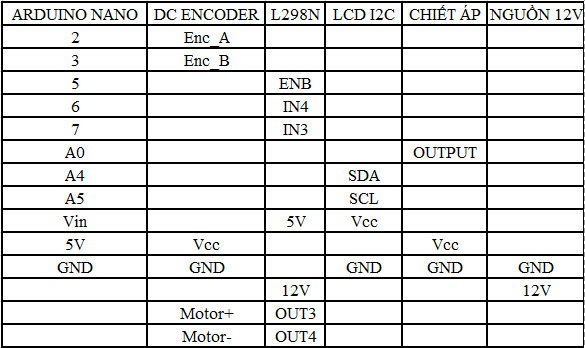
\includegraphics[width=0.8\textwidth]{sd2.png}
	\caption[Sơ đồ chân nối mô hình điều khiển vị trí góc quay động cơ DC Encoder]{Sơ đồ chân nối mô hình điều khiển vị trí góc quay động cơ DC Encoder}
	\label{fig:Sơ đồ chân nối mô hình điều khiển vị trí góc quay động cơ DC Encoder}
\end{figure}




%\include{Appendices/AppendixC}

%----------------------------------------------------------------------------------------

\end{document} 
%----------------------------------------------------------------------------------------------------------------------------------------
